\documentclass[times,english,brazil,oneside,a4paper,fleqn]{ifes8}

\usepackage[utf8]{inputenc}
\usepackage[T1]{fontenc}
\usepackage{lastpage}           
\usepackage[alf]{abntex2cite}
\usepackage{microtype}          
\usepackage{morefloats}        
\usepackage{listings}
\usepackage{xcolor}
\usepackage{tikz}
\usepackage{hyperref}
\usetikzlibrary[topaths]
\usepackage{mathtools}
\usepackage[final]{pdfpages}
\usepackage{caption}
\usepackage{subcaption}
\usepackage{multirow}
\usepackage{hhline}
\usepackage{boxhandler}
\usepackage[normalem]{ulem}
\usepackage{dirtytalk}
\usepackage{float}
\usepackage{siunitx}
\usepackage{svg}
\usepackage[none]{hyphenat}
\usepackage{breqn}
\usepackage{upgreek}
\usepackage{makecell}
\usepackage{amsmath}
\usepackage[toc, acronym]{glossaries}
\usepackage{chngcntr}
\usepackage{attachfile}
\usepackage{imakeidx}
\usepackage{svg}
\hyphenation{es-ta-be-le-ci-men-to}
\usepackage{tabularx}
\raggedbottom
\selectlanguage{brazil}
\setlength{\abovecaptionskip}{5pt}


%%% Define que todos os códigos fontes construídos com o ambiente
%%% `lstlisting' terão uma borda simples.
\lstset{ %
  backgroundcolor=\color{white},   % choose the background color
  basicstyle=\footnotesize,        % size of fonts used for the code
  breaklines=true,                 % automatic line breaking only at whitespace
  captionpos=b,                    % sets the caption-position to bottom
  commentstyle=\color{mygreen},    % comment style
  escapeinside={\%*}{*)},          % if you want to add LaTeX within your code
  keywordstyle=\color{blue},       % keyword style
  stringstyle=\color{mymauve}, 
  numbers=left,
  stepnumber=1,    
  firstnumber=1,
  numberfirstline=true% string literal style,
   frame=top,frame=bottom, frame=single,
   captionpos=t,
   literate=
  {á}{{\'a}}1 {é}{{\'e}}1 {í}{{\'i}}1 {ó}{{\'o}}1 {ú}{{\'u}}1
  {Á}{{\'A}}1 {É}{{\'E}}1 {Í}{{\'I}}1 {Ó}{{\'O}}1 {Ú}{{\'U}}1
  {à}{{\`a}}1 {è}{{\`e}}1 {ì}{{\`i}}1 {ò}{{\`o}}1 {ù}{{\`u}}1
  {À}{{\`A}}1 {È}{{\'E}}1 {Ì}{{\`I}}1 {Ò}{{\`O}}1 {Ù}{{\`U}}1
  {ä}{{\"a}}1 {ë}{{\"e}}1 {ï}{{\"i}}1 {ö}{{\"o}}1 {ü}{{\"u}}1
  {Ä}{{\"A}}1 {Ë}{{\"E}}1 {Ï}{{\"I}}1 {Ö}{{\"O}}1 {Ü}{{\"U}}1
  {â}{{\^a}}1 {ê}{{\^e}}1 {î}{{\^i}}1 {ô}{{\^o}}1 {û}{{\^u}}1
  {Â}{{\^A}}1 {Ê}{{\^E}}1 {Î}{{\^I}}1 {Ô}{{\^O}}1 {Û}{{\^U}}1
  {œ}{{\oe}}1 {Œ}{{\OE}}1 {æ}{{\ae}}1 {Æ}{{\AE}}1 {ß}{{\ss}}1
  {ű}{{\H{u}}}1 {Ű}{{\H{U}}}1 {ő}{{\H{o}}}1 {Ő}{{\H{O}}}1
  {ç}{{\c c}}1 {Ç}{{\c C}}1 {ø}{{\o}}1 {å}{{\r a}}1 {Å}{{\r A}}1
  {€}{{\EUR}}1 {£}{{\pounds}}1
}

\newcommand{\ifestex}{\textsf{Ifes$8$}}

\newcolumntype{C}{>{\centering\arraybackslash}X}

\def\tituloDoTrabalho{Um Estudo das Consequências da Compressão de Arquivos Multimídia em Diferentes Contextos de Imagem}
\autor{Bruno da Fonseca Chevitarese \and Luiz Felipe Elizeta}  % Para separar autores use  \and

\def\nomeCurso{Curso Superior de Bacharelado em Sistemas de Informação}
\def\nomeOrientador{Flávio Giraldeli}
\def\tituloOrientador{Prof. Me.}
\def\tipoDeTrabalho{Trabalho Acadêmico para Acompanhamento de Disciplina}
\def\nomeInstituicao{Instituto Federal de Educação, Ciência e Tecnologia do Espírito Santo}

\local{Serra}
\data{2024}

\preambulo{Este trabalho tem por finalidade validar os conhecimentos adquiridos pelos alunos durante as aulas da Disciplina Fundamentos de Sistemas Multimídia.}


% INFORMAÇÕES PARA ERRATA
\def\localDefesa{LOCAL}
\def\dataDefesa{DATA}
\def\nomeAutores{Sobrenome, Nome}
% INFORMAÇÕES PARA ERRATA

% Informações Fixas
\titulo{\tituloDoTrabalho}
\curso{\nomeCurso}
\orientador[Orientador:]{\tituloOrientador \nomeOrientador}

\tipotrabalho{\tipoDeTrabalho}
\instituicao{\nomeInstituicao}
\autorficha{}
\newcommand{\fonteElementoGrafico}[1]{
    \vspace{0.3cm}
    \small
    Fonte: #1
}

\newcommand{\autoriaPropria}{
    \fonteElementoGrafico{Autoria própria}
}

\newcommand{\paragrafo}{
    \hspace{1.5 cm}
}

\newcommand{\indice}[1]{
    #1\index{#1}
}
\counterwithin{table}{chapter}
\counterwithin{figure}{chapter}

% \makeglossaries

\newglossaryentry{bit}{
    name=,
    description={
    
    },
    plural=
}

% \makeindex[columns=3, intoc, title=ÍNDICE, options= -s Configurações/IndiceAlfabetico.ist] % CASO QUERIA CRIAR UM ÍNDICE

% ----------------------------------------------------------
% Documento
% ----------------------------------------------------------

\begin{document}

\setsecnumformat{\csname the#1\endcsname\space}
\renewcommand{\afterchapternum}{\hspace{-4pt}}
    
\imprimircapa
 \addtocounter{page}{-1}
    
\imprimirfolhaderosto*
    
\addtocounter{page}{-1}

    
% ----------------------------------------------------------
% ELEMENTOS PRÉ-TEXTUAIS (aqueles que estiverem comentados não são obrigatórios)
% ----------------------------------------------------------

% \begin{resumo}[ERRATA]
    \vspace*{-6mm}
    
    \nomeAutores. \textbf{\tituloDoTrabalho}. \tipoDeTrabalho \space-- \nomeCurso, \nomeInstituicao, \localDefesa, \dataDefesa.

    
    \begin{table}[htbp]
    \centering

    \begin{tabularx}{\textwidth}{C|C|C|C}
        \hline
        
        \textbf{Folha} & \textbf{Linha} & \textbf{Onde se lê} & \textbf{Leia-se} \\ \hline
        
        
    \end{tabularx}
    \end{table}

    
\end{resumo}

% \begin{resumo}[AGRADECIMENTOS]
\vspace*{-6mm}
    
    Texto Aqui
    
\end{resumo}

% \begin{epigrafe}
  \vspace*{20cm}
  \begin{otherlanguage}{english}
    \begin{flushright}
      \begin{SingleSpace}
		\textit{HERE} \\
		(NAME)
      \end{SingleSpace}
    \end{flushright}
  \end{otherlanguage}
\end{epigrafe}


\renewcommand{\afterloftitle}{\null\\[5mm]}
\renewcommand{\afterlottitle}{\null\\[5mm]}
\renewcommand{\afterloqtitle}{\null\\[5mm]}
\renewcommand{\aftertoctitle}{\null\\[5mm]}
% TODOS AQUI SÃO OPICIONAIS, MAS É VÁLIDO MANTÊ-LOS
\renewcommand{\listfigurename}{LISTA DE FIGURAS}
\pdfbookmark[0]{\listfigurename}{lof}
\listoffigures*
\cleardoublepage

\pdfbookmark[0]{\listadequadrosname}{loq}
\listadequadros*
\cleardoublepage

\renewcommand{\listtablename}{LISTA DE TABELAS}
\pdfbookmark[0]{\listtablename}{lot}
\listoftables*
\cleardoublepage


% TODOS AQUI SÃO OPICIONAIS, MAS É VÁLIDO MANTÊ-LOS


\renewcommand{\contentsname}{SUMÁRIO}
\pdfbookmark[0]{\contentsname}{toc}
\tableofcontents*
\cleardoublepage

% ----------------------------------------------------------
% ELEMENTOS TEXTUAIS
% ----------------------------------------------------------
\textual
\captionsetup{justification=justified,singlelinecheck=false}



    % ----------------------------------------------------------
    % Desenvolvimento
    \captionsetup{justification=centering,margin=0cm}
\label{cap:atividade1}  % Forma de referenciar o capítulo no comando \ref

%inicio do capitulo
\chapter[Atividade 1: ENTENDENDO IMAGENS VETORIAIS E \textit{BITMAPS}]{Atividade 1: ENTENDENDO IMAGENS VETORIAIS E \textit{BITMAPS}}

Como é sabido, pode-se dividir as imagens em dois tipos distintos: imagens vetoriais e imagens \textit{bitmap}. Ambas possuem as suas características e utilidades e essa seção busca explicitar essas diferenças.

\section{Conceituando imagens \textit{bitmaps} e vetoriais}

A priori, pode-se entender uma imagem em \textit{bitmap} como uma matriz com "I" linhas, "J" colunas e "K" canais. Cada elemento dessa matriz é um \textit{pixel}, unidade fundamental de composição de imagens, composto por um vetor "K" que varia de acordo com o formato do arquivo.

\hspace{1.5 cm} Uma imagem vetorial, por outro lado, consiste em uma fórmula matemática que gera uma imagem. Essa função recebe como parâmetro a escala utilizada, então o computador renderiza a imagem a partir desses parâmetros e dessa função. Inclusive, esse PDF possui fontes vetoriais!

\hspace{1.5 cm} Como pode-se perceber, ambas as imagens são feitas de forma diferentes, logo é de se esperar que elas possuam características distintas. No geral, imagens em \textit{bitmap} são mais indicadas em situações onde é preciso muitas informações. Fotos do mundo real, por exemplo, são feitas em \textit{bitmap}; o problema disso é que além delas serem costumeiramente mais "pesadas" que imagens vetoriais, a ampliação da imagem implica na redução da qualidade da imagem. Já imagens vetoriais, por serem fórmulas, costumam ser mais leves (mas depende da quantidade de detalhes que a imagem busca ter) e o zoom nela não perde qualidade.

\subsection{SVG, Composição Interna}
Existem muitos tipos de arquivos de imagem. O tipo escolhido para fazer essa atividade é o SVG (\textit{Scalable Vector Graphics}) muito utilizado no contexto do desenvolvimento \textit{web}. Antes de analisar as imagens, deve-se compreender a sua estrutura. Para fazer essa análise, utilizou-se o editor de texto "Notepad++".

\hspace{1.5 cm} Assim como muitos outros arquivos de imagem, o SVG inicia com um cabeçalho (\textit{header}) que contém algumas informações básicas sobre ele. Depois, uma série de comando são utilizados, seguindo uma sintaxe semelhante à nossa linguagem de marcação favorita, o HTML5 (Linguagem de Marcação de Hipertexto). Curiosos, decidimos fazer algumas pesquisas e descobrimos que existe uma \textit{tag} no HTML5 chamada svg. Ou seja, basta "ligar o tico no teco", uma imagem SVG nada mais é do que uma composição da tag svg do HTML, expandida para um arquivo separado na composição da página, justificando o seu vasto uso no contexto web.

\section{Percepções Sobre Imagens Vetoriais}
Utilizou-se 5 imagens para fazer observações sobre esse tipo de composição. Como esperado o zoom na imagem não influencia na qualidade. Ademais, como esperado, as imagens não possuem textura. Se for analisado com cautela, pode-se perceber que conceitos como luz e sombra são aplicados, assim como variações de tons e degradês. Contudo, por se tratar de um desenho essencialmente, as imagens possuem cores sólidas preenchendo totalmente o espaço. Isso não costuma ser um problema, mas se observar a Imagem \ref{fig:carro} você há de notar como é esquisito esse carro.

\begin{figure}[h!]
    \centering
    \caption{Carro no formato SVG}
    \label{fig:carro}
    
    \includesvg[scale=0.1]{Documeto/1-ElementosTextuais/1-Desenvolvimento/imagens-atividade1/NewTux.svg}

    \fonteElementoGrafico{Fornecido pelo Professor}
    
\end{figure}

\hspace{1.5 cm} Acreditamos que essa sensação aconteça nessa figura em particular por dois motivos. O primeiro é que essa imagem propõe-se a parecer mais realista, trazendo muito a percepção de luz e sombra, o que faz o cérebro buscar por outras informações que não existem. A segunda é porque a imagem traz um carro, objeto tão familiarizado por nós que nos força a buscar informações mais realistas nele. 

\section{Comparando Imagens Vetoriais e \textit{Bitmaps}}
Já foi explicado a diferença entre os dois tipos de imagem. Agora, vamos explicitar a diferença entre elas. Abaixo, seguem as Imagens \ref{fig:carro_png} e \ref{fig:carro_SVG}.

\begin{figure}[h!]
    \centering
    \caption{Carro no formato PNG}
    \label{fig:carro_png}
    
    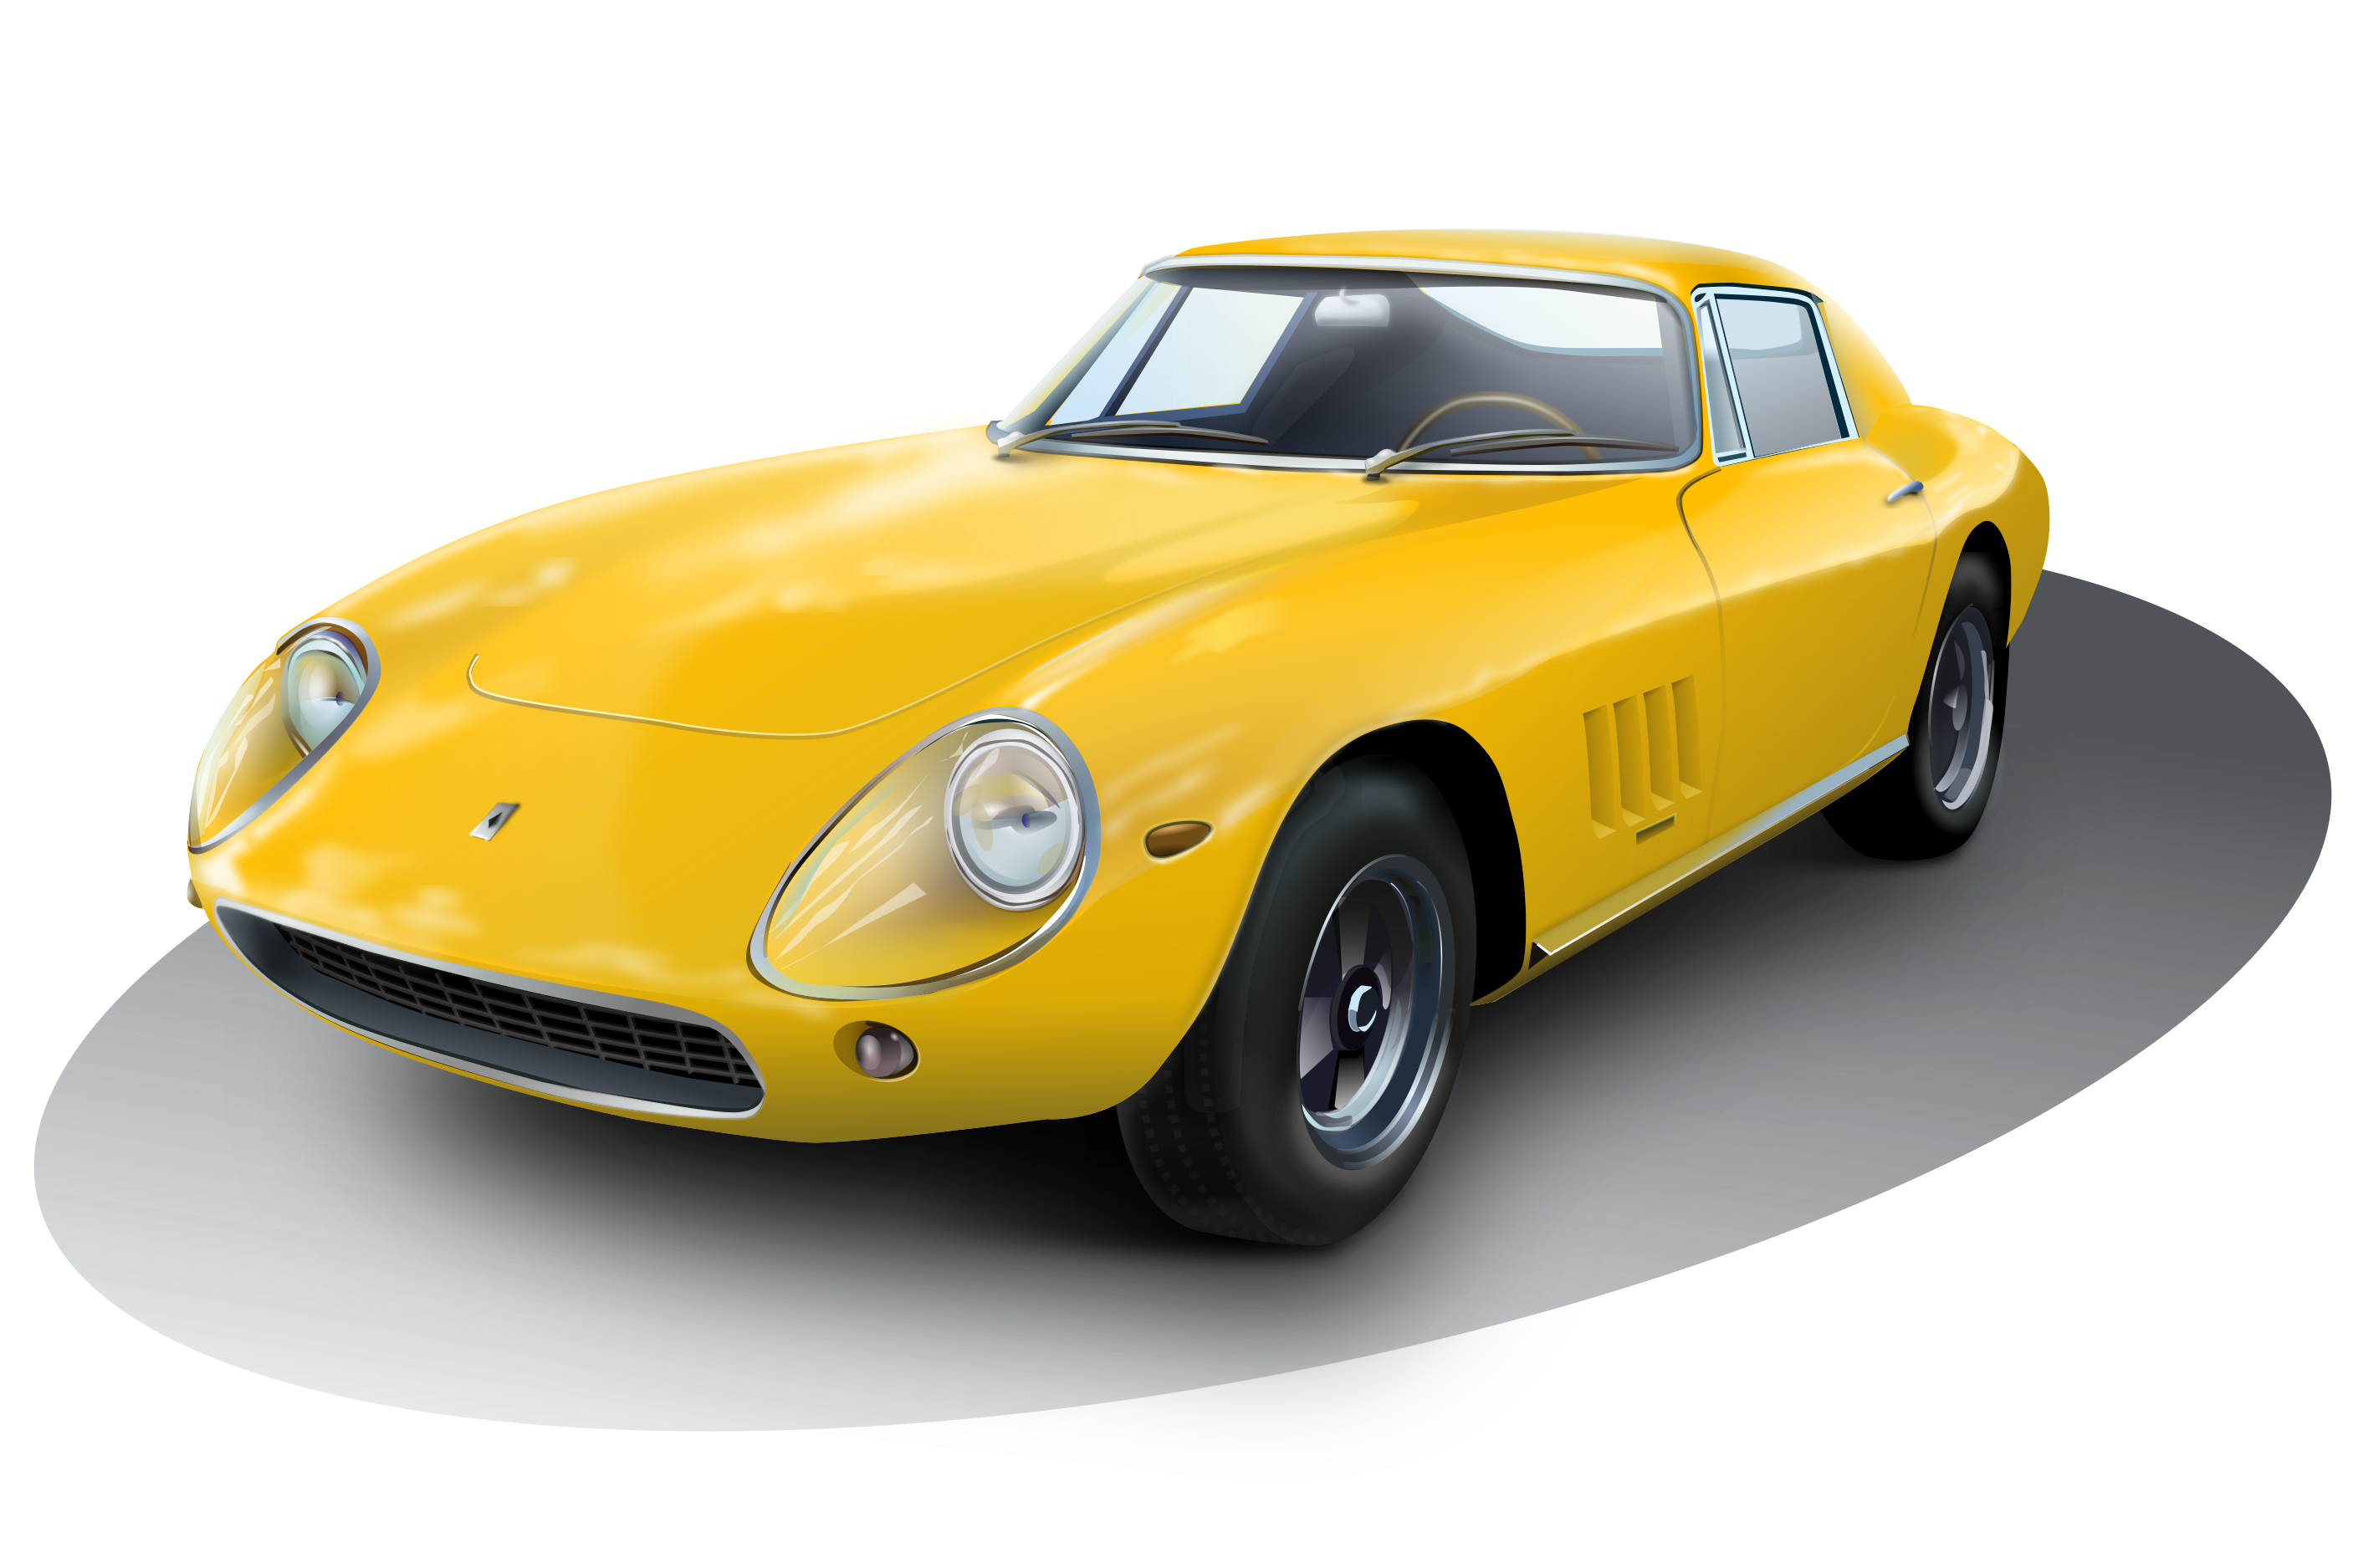
\includegraphics[scale=0.1]{Documeto/1-ElementosTextuais/1-Desenvolvimento/imagens-atividade1/car.png}

    \fonteElementoGrafico{Fornecido pelo Professor}
    
\end{figure}

\begin{figure}[h!]
    \centering
    \caption{Carro no formato SVG}
    \label{fig:carro_SVG}
    
    \includesvg[scale=0.1]{Documeto/1-ElementosTextuais/1-Desenvolvimento/imagens-atividade1/NewTux.svg}

    \fonteElementoGrafico{Fornecido pelo Professor}
    
\end{figure}

\hspace{1.5 cm} Escolheu-se essa imagem, pois, ela possui mais detalhes, o que a torna melhor para fazer esse tipo de comparação. Após converter a imagem para PNG já pode ser observado uma diferença, o tamanho da imagem aumentou quase 3,5$\times$. Depois, apenas as diferenças já explicitadas, a questão da perda de qualidade ao realizar o zoom. Para melhor exemplificar isso, seguem as Imagens \ref{fig:farol_carro_svg} e \ref{fig:farol_carro_png}.

\begin{figure}[h!]
    \centering
    \caption[Caption for LOF]{Farol do carro em SVG, zoom 500\% \footnotemark}
    \label{fig:farol_carro_svg}
    
    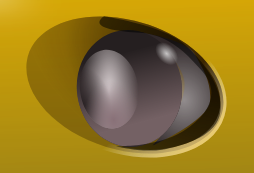
\includegraphics[scale=0.7]{Documeto/1-ElementosTextuais/1-Desenvolvimento/imagens-atividade1/farol_car_svg.png}

    \fonteElementoGrafico{Fornecido pelo Professor}
    
\end{figure}
\footnotetext{Zoom renderizado no navegador \textit{Firefox}}

\begin{figure}[h!]
    \centering
    \caption[Caption for LOF]{Farol do carro em png, zoom 500\%\footnotemark}
    \label{fig:farol_carro_png}
    
    
\includegraphics[scale=0.3]{Documeto/1-ElementosTextuais/1-Desenvolvimento/imagens-atividade1/farol_car_png.png}

    \fonteElementoGrafico{Fornecido pelo Professor}
    
\end{figure}
\footnotetext{Zoom renderizado pelo aplicativo \textit{Photoshop}CS5 (obviamente obtido legalmente). Escolhemos esse \textit{software} para evitar filtros que outros aplicativos possam vir a utilizar ao dar zoom.}
    \captionsetup{justification=centering,margin=0cm}
\label{cap:atividade2}  % Forma de referenciar o capítulo no comando \ref

%inicio do capitulo
\chapter[Atividade 2 - Comparando diferentes subsamplings]{Atividade 2 - Comparando diferentes subsamplings}
Neste capítulo iremos realizar uma atividade um tanto um quanto peculiar, iremos utilizar o programa para análise de \textit{DownSampling}/\textit{SubSampling} em vídeo observando um arquivo sem compressão.

\section{Compreendendo melhor as informações fornecidas pelos arquivo}
Ao utilizar o software AvarexYUVPlayer com as seguintes configurações, evidenciadas na Figura \ref{fig:imagem8}:

\begin{figure}
    \centering
    \caption{Tela o software AvarexYUVPlayer}
    \label{fig:imagem8}
    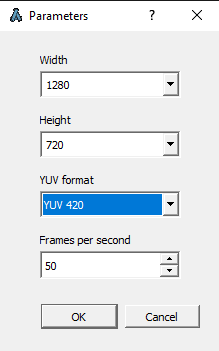
\includegraphics{Documeto/1-ElementosTextuais/images/08.png}

    \autoriaPropria
\end{figure}

\paragrafo Sendo o parâmetro de resolução crítico para visualização do video. Podemos analisar os efeitos do \textit{subsampling} em video, o que sinceramente alterou em nada na visualização do vídeo.

\paragrafo Ao tentar comprimir estes arquivos em RAR, ZIP e 7Z, foi-se obtidos resultados pouco satisfatórios, o ratio variou pouco entre os arquivos e esperávamos mais do 7Z, que exige um esforço computacional enorme e entrega algo ligeiramente melhor que os demais. Isto é, o ocorrido provavelmente se dá pelo software não ser capaz de aproveitar a pouca variação temporal, não tratam com eficiência vídeos no geral por conta disso.

obs: Não conseguimos fazer os cálculos para encontrar o valor exato do arquivo.


\section{Avaliando a influência dos parâmetros nos vídeos}
Em cada arquivo apenas varia o Subsampling, alterando “proporcionalmente” o tamanho do arquivo, mas sem alterar a qualidade, isso se deve ao fato de que subsampling é basicamente uma redução lossy de informações de luminância, informação essa que o ser humano não possui sensibilidade, passando despercebida. Além de que, por se tratar de um vídeo, é ainda mais complicado de perceber a diferença visto que não conseguimos analisar uma imagem por tempo o suficiente para separarmos as cores, causando uma mistura ainda maior e uma menor percepção de alterações de cores.
    \captionsetup{justification=centering,margin=0cm}
\label{cap:atividade3}  % Forma de referenciar o capítulo no comando \ref

%inicio do capitulo
\chapter[Atividade 3 - Analisando as características dinâmicas do vídeo]{Atividade 3 - Analisando as características dinâmicas do vídeo}

A seguinte atividade busca evidenciar a teoria através da prática. Ao analisarmos diferentes vídeos, com conteúdos, formatos e taxa de frames diferentes, pretende-se esclarecer onde a teoria encontra a prática.

\section{Vídeo 1 - Um vídeo em Slow Motion}
Pode-se abstrair um vídeo em slow motion como uma gravação a um FPS muito elevado exibido a um FPS baixo. Ou seja, suponha um vídeo gravado em 60 quadros por segundo. Se exibirmos ele a 30 quadros por segundo teremos a impressão de que as coisas estão mais lentas, isso porque um movimento que originalmente demoraria 1 segundo para ser concluído agora demora 2. É importante destacar isso, pois esse fato tem influência direta na redundância temporal do vídeo.

\paragrafo Como explicado pela teoria, a compressão de vídeo deve levar em consideração dois fatores: a redundância espacial e a redundância temporal. Em relação à redundância espacial, todos os conceitos de imagem são aplicados (afinal de contas, vídeos são compostos por imagens), ou seja, na redundância espacial busca-se comprimir uma imagem de uma forma inteligente o suficiente. No entanto, isso só é válido para os key frames, também chamados de quadros chave ou intra frames; nos demais, busca-se uma forma de otimizar o tamanho do vídeo. Para tal, uma série de técnicas são aplicadas a fim de aproveitar regiões que mantiveram-se estáticas para fazer a construção da próxima imagem.

\paragrafo Um vídeo em slow motion é perfeito para exemplificar a redundância temporal. Considerando o exemplo onde um movimento de 1 segundo é executado em 2 segundos, há uma maior suavidade no movimento. Assim, a distância entre um frame e outro é bem menor do que no caso original. Como pode ser observado na imagem abaixo, os vetores indicadores de movimento são muito pequenos, mesmo em cenas com grande movimentação.

\begin{figure}[H]
    \centering
    \caption{Imagem do vídeo em \textit{slowmotion}}
    \label{fig:imagem9}
    
    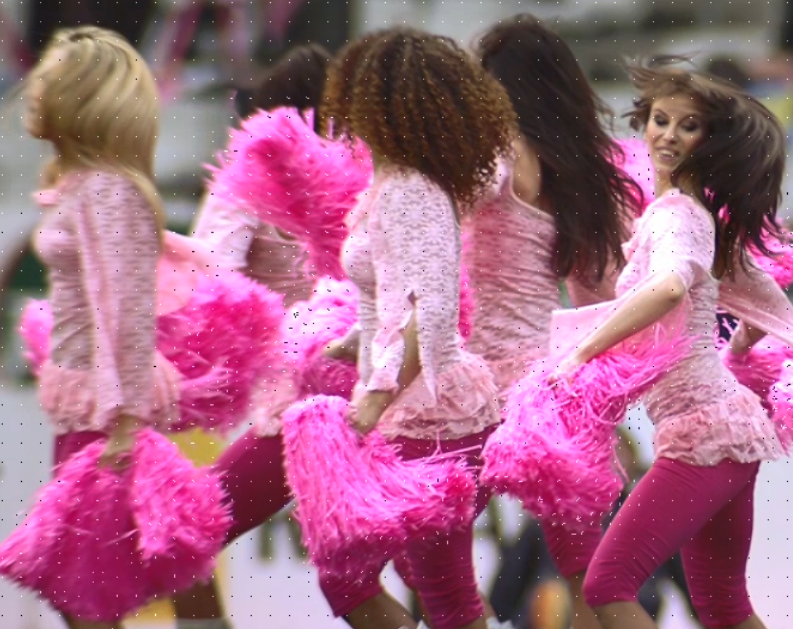
\includegraphics[scale=0.5]{Documeto/1-ElementosTextuais/images/09.png}

    \small
    Extraído dos vídeos fornecidos pelo Professor
\end{figure}

\paragrafo Outra coisa importante em relação a esse vídeo é a distribuição de frames do tipo I, B e P. No pseudo gráfico abaixo é possível identificar pontos de pico. Esses pontos de pico indicam quadros do tipo I. Como a composição do vídeo em slow motion é constituída por menos movimentos, o codec usa os I frames em momentos onde o acúmulo de perdas em relação a outros quadros é muito grande, ou em momentos específicos limitados por flags do arquivo. Repare que na maior parte do tempo, a segunda forma se faz verdadeira, mas há momentos, geralmente nas transições entre cenas, que o codec é obrigado a usar um frame tipo I para evitar maiores perdas.

\paragrafo Além disso, algo interessante ocorre no uso de quadros B e P. A proporção média é de um para um, isto é, um quadro P e um quadro B. Baseado nos nossos testes realizados de forma empírica, momentos de vídeos com maior redundância temporal costumam ter mais frames do tipo B do que a média se comparados a outros trechos do mesmo vídeo. No trecho do filme “The Matrix”, analisado na próxima sessão, há pouca presença de quadros B. No caso do arquivo em slow motion, a relação com a teoria encontrada foi que como a diferença entre um quadro no índice x em relação ao índice x+2 é tão pequena que a taxa de erro da composição também fica muito pequena, tornando viável seu uso do quadro tipo B no índice x+1.

\begin{figure}[H]
    \centering
    \caption{Imagem do vídeo em \textit{slowmotion}}
    \label{fig:imagem10}
    
    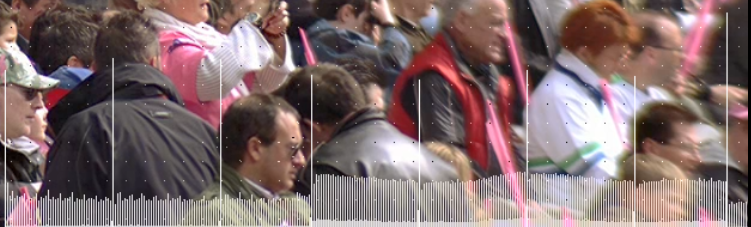
\includegraphics[scale=0.5]{Documeto/1-ElementosTextuais/images/10.png}

    \small
    Extraído dos vídeos fornecidos pelo Professor
\end{figure}

\paragrafo As informações importantes ainda não acabaram. O bitrate acompanha a complexidade da imagem analisada no momento, o que faz todo sentido. Sendo o bitrate a taxa de transferência de dados para a renderização do vídeo, faz sentido que imagens mais complexas exigirem uma maior taxa de transferência. No caso, os trechos mais pesados são os key frames, enquanto a complexidade dos demais é definida pela redundância temporal. Por exemplo, em cenas muito movimentadas, a tendência é que um bitrate maior seja exigido.

\section{Vídeo 2 - Cena Aleatória de The Matrix (1999)}

Boa parte das observações feitas na sessão anterior são válidas nesta sessão. No entanto, essa cena diferencia-se pela forma como foi gravada, que é no tempo normal. Além disso, a cena por si só é extremamente movimentada, com bolsa para lá e pra cá, tiro para todo lado, personagens andando, coadjuvantes morrendo, e zás e zás. Como pode-se perceber, a natureza da cena variou muito de uma análise para outra, assim é mais proveitoso interpretar as diferenças entre os vídeos do que ficar repetindo “mais do mesmo”.

\paragrafo A primeira coisa a se notar é que a imagem do vídeo em questão tem uma paleta de cores na cena mais escura e puxada para o verde se comparado ao vídeo em slow motion. Ou seja, a compressão da imagem é mais perceptível ao olho humano do que se a informação estivesse em regiões mais claras; o que implica na perda de transparência da imagem com mais facilidade. Isso influencia diretamente no bitrate necessário na descompressão. Isto é apenas um detalhe, mas não deixa de ser importante comentar.

\paragrafo Ademais, perceba que a quantidade de informação temporal dessa cena é muito maior do que a do vídeo em \textit{slowmotion}. A Figura \ref{fig:imagem11} demonstra isso com clareza. Nela, há uma vasta quantidade de \textit{motion vercotrs}, o que indica a movimentação das informações na cena, e por sua vez acumula informação. Isso influencia diretamente no bitrate, bem como na presença dos \textit{frames} tipo P e B.

\begin{figure}[H]
    \centering
    \caption{Imagem do filme \textit{The Matrix}}
    \label{fig:imagem11}
    
    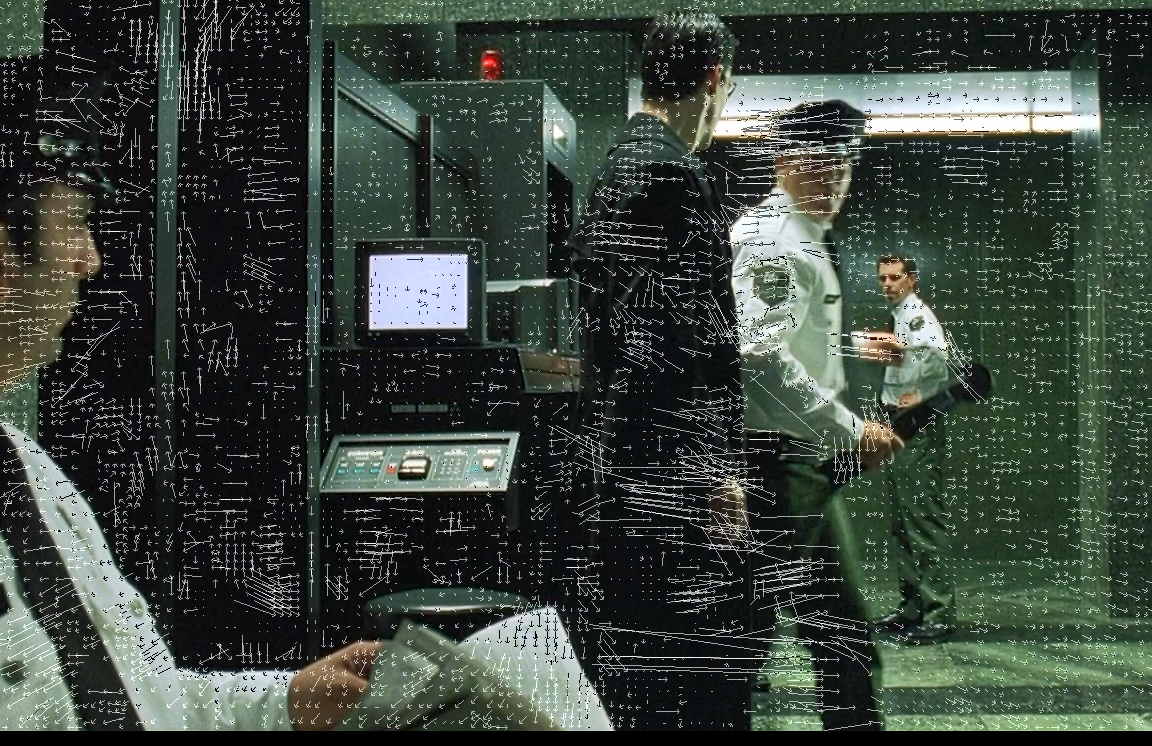
\includegraphics[scale=0.3]{Documeto/1-ElementosTextuais/images/11.png}

    \small
    Extraído dos vídeos fornecidos pelo Professor
\end{figure}

\paragrafo A Figura \ref{fig:imagem12} demonstra quais \textit{frames} o encoder optou por utilizar. Diferente do vídeo em \textit{slowmotion}, o trecho do filme não tão bem comportado. Os \textit{frames} tipo I não estão tão espaçados com a mesma constância que os \textit{frames} do vídeo anterior. Outra coisa que pode ser observadas é que esse tipo de quadro aparece em transições de cena. Além disso, há momentos de constância muito grande de frames tipo P, que são os momentos de uma "onda contínua", enquanto os \textit{frames} tipo B aparecem bem menos, em locais de "altura" menor. 

\begin{figure}[H]
    \centering
    \caption{Imagem do filme \textit{The Matrix}}
    \label{fig:imagem12}
    
    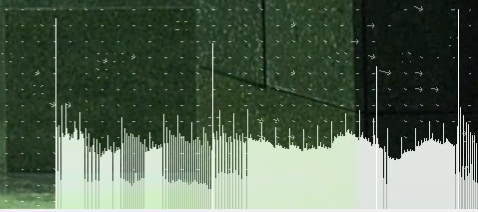
\includegraphics[scale=1]{Documeto/1-ElementosTextuais/images/12.png}

    \small
    Extraído dos vídeos fornecidos pelo Professor
\end{figure}


\section{Vídeo 3 - Último Episódio da Temporada 4 de \textit{Game of Thrones}}
Agora, é o momento de preparar uma pipoca e analisar um episódio longo de uma série mais longa ainda. Como o episódio é muito extenso não iremos comentar ele todo. Ao invés disso, vamos separar trechos interessantes de serem anualizados baseado nos conhecimentos então adquiridos.


\subsection{Um começo caótico}
Primeiramente, vamos analisar a tão famosa abertura da série. No primeiro momento, temos a logo da HBO Entretairement. Essa vinheta inicia-se com um ruído muito intenso, o que aumenta muito o bitrate nesse momento. Como demonstra a Figura \ref{fig:imagem12}, a construção da imagem é de alta complexidade espacial, apesar da pouca complexidade temporal.

\begin{figure}[H]
    \centering
    \caption{Imagens da abertura do episódio citado de \textit{Game of Trhones}}
    \label{fig:imagem13-14-15}
    
    
\includegraphics[scale=0.33]{Documeto/1-ElementosTextuais/images/13.png}
    
\includegraphics[scale=0.25]{Documeto/1-ElementosTextuais/images/14.png}

    \small
    Extraído dos vídeos fornecidos pelo Professor
\end{figure}

\paragrafo Então, a abertura da série é exibida e ela tem, de forma geral, uma complexidade bem maior que o resto do episodio, já que o seu \textit{bitrate} foi consideravelmente maior que a média. Isso ocorre devido a dois fatores: primeiro, a complexidade espacial dela é bem grande, com muitas formas bem definidas e regiões com bastante "textura"; a segunda é que a complexidade temporal em toda a cena é bastante constate -- geralmente, uma cena pode ter complexidade temporal alta, mas costuma ser em pontos específicos na tela, ou no cenário ou em um objeto, já na abertura a cena como um todo tem movimento.


\subsection{Cenas escuras}
A Figura \ref{fig:imagem17} traz outra cena do episódio. Enquanto a abertura era bem mais complexa, esse trecho é mais simples. Apesar da correção de movimento ser muito intensa, a forma como a câmera constrói a cena permite muita redundância nas informações.

\begin{figure}[H]
    \centering
    \caption{Imagem do início do episódio citado de \textit{Game of Trhones}}
    \label{fig:imagem17}
    
    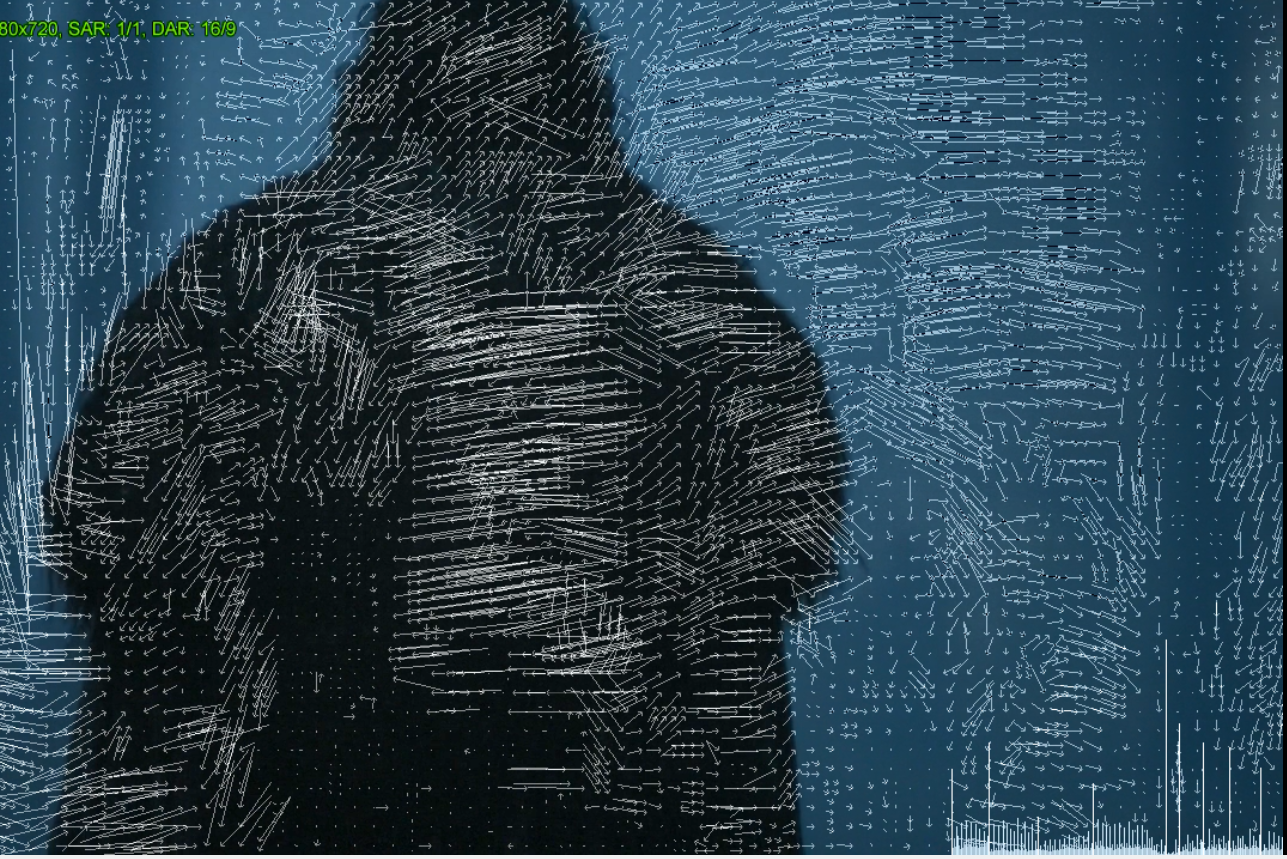
\includegraphics[scale=0.35]{Documeto/1-ElementosTextuais/images/17.png}

    \small
    Extraído dos vídeos fornecidos pelo Professor
\end{figure}

\paragrafo Além disso, cenas que tem um ritmo mais lento tem um gráfico de complexidade mais comportado. Em comparação a cenas mais claras, os artefatos são muito evidentes nos trechos mais escuros, como demonstrado na Figura \ref{fig:imagem18}

\begin{figure}[H]
    \centering
    \caption{Imagem do episódio citado de \textit{Game of Trhones}}
    \label{fig:imagem18}
    
    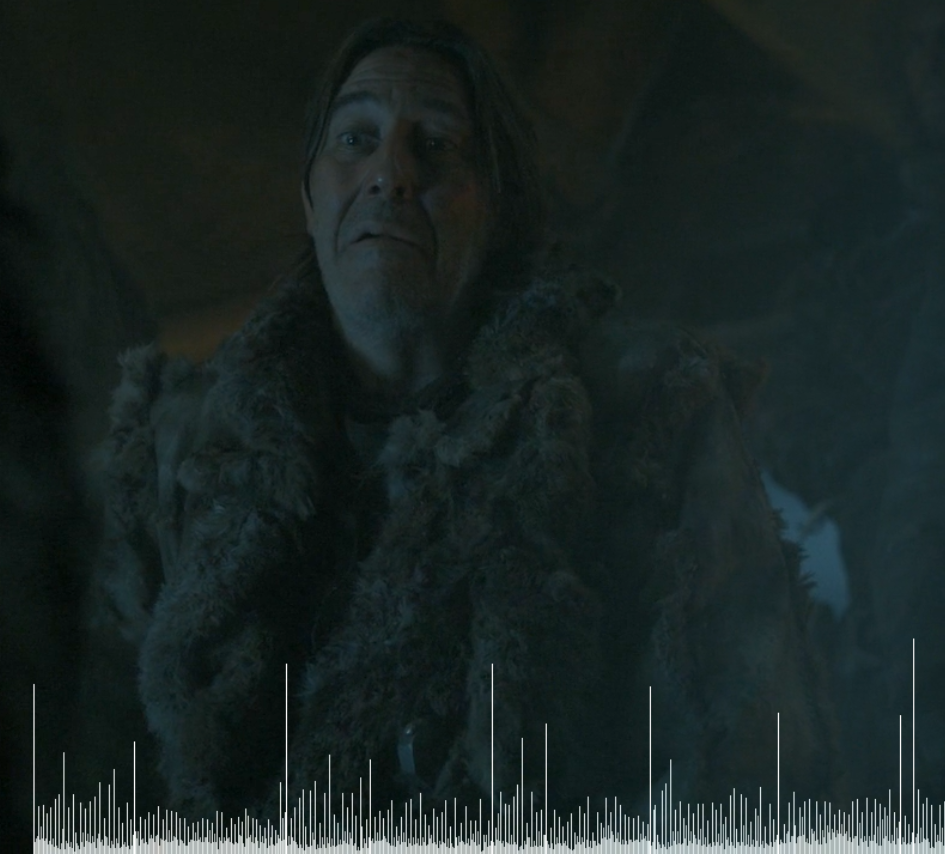
\includegraphics[scale=0.35]{Documeto/1-ElementosTextuais/images/18.png}

    \small
    Extraído dos vídeos fornecidos pelo Professor
\end{figure}


\subsection{Cenas Claras}
Em cenas claras um comportamento semelhante pode ser observado. Regiões mais escuras tem artefatos bastante visíveis, enquanto regiões mais claras são mais transparentes. Além disso, momentos mais calmos apresentam gráficos mais comportados.

\begin{figure}[H]
    \centering
    \caption{Imagem do episódio citado de \textit{Game of Trhones}}
    \label{fig:imagem19}
    
    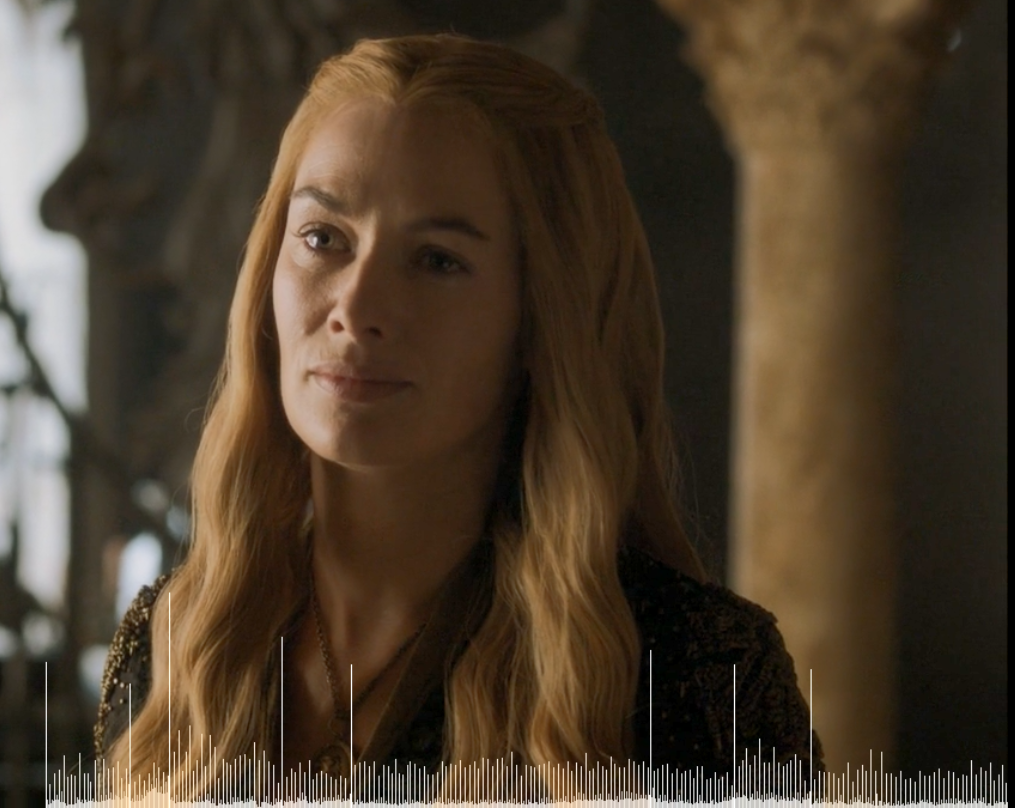
\includegraphics[scale=0.35]{Documeto/1-ElementosTextuais/images/19.png}

    \small
    Extraído dos vídeos fornecidos pelo Professor
\end{figure}

\paragrafo Além disso, é muito interessante perceber como a iluminação artificial e a iluminação natural tem grande influência na percepção dos artefatos e também no comportamento da complexidade da cena. Quando a iluminação é artificial, os artefatos são mais perceptíveis e a transição entre camadas é bem mais suave, valorizando a cena. Além disso, em cenas com iluminação artificial é comum perceber que há uma variância muito brusca na correção de movimento mesmo que as personagens estejam paradas, o que é justificado pelo fato da iluminação artificial "piscar" ao invés de emitir de fato luz.


\begin{figure}[H]
    \centering
    \caption{Imagem do episódio citado de \textit{Game of Trhones} (supostamente em iluminação artificial); a imagem da direita é o exato frame posterior ao frame da esquerda}
    \label{fig:imagem20-21}
    
    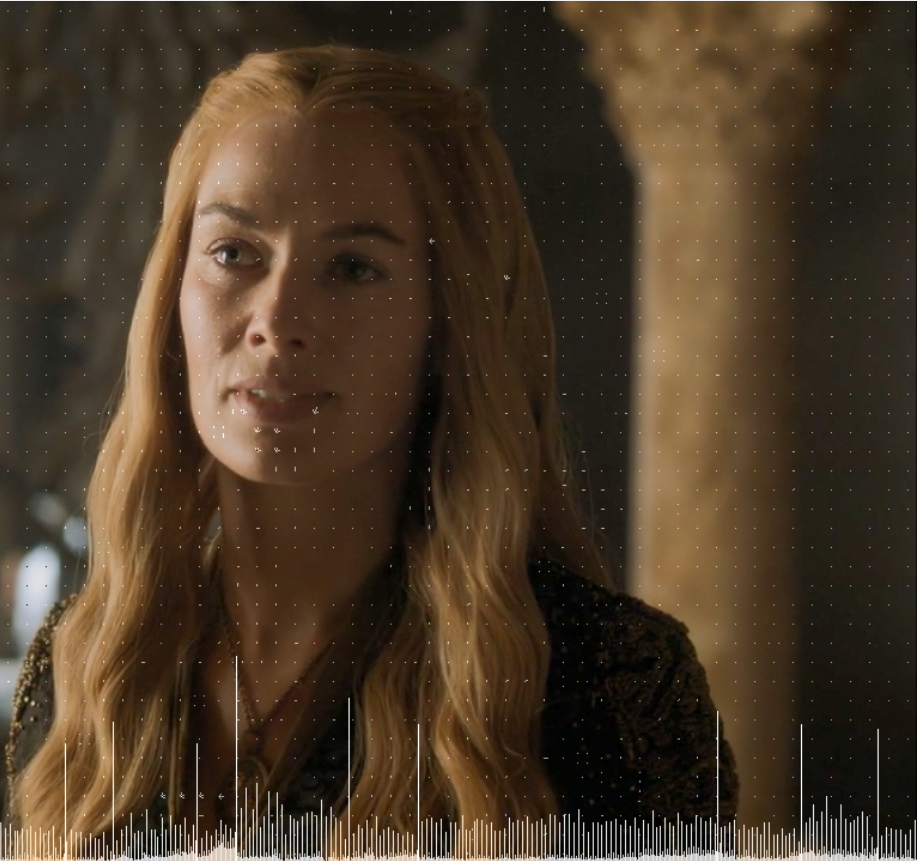
\includegraphics[scale=0.3]{Documeto/1-ElementosTextuais/images/20.png}
    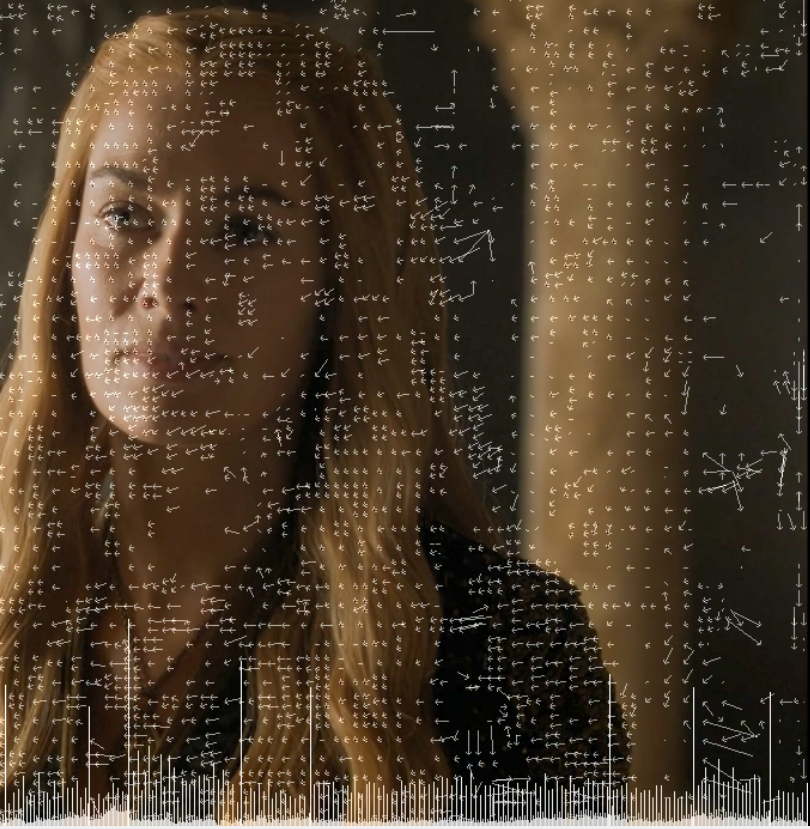
\includegraphics[scale=0.3]{Documeto/1-ElementosTextuais/images/21.png}

    \small
    Extraído dos vídeos fornecidos pelo Professor
\end{figure}


\begin{figure}[H]
    \centering
    \caption{Imagem do episódio citado de \textit{Game of Trhones} (supostamente em iluminação natural); a imagem da direita é o exato frame posterior ao frame da esquerda}
    \label{fig:imagem22-23}
    
    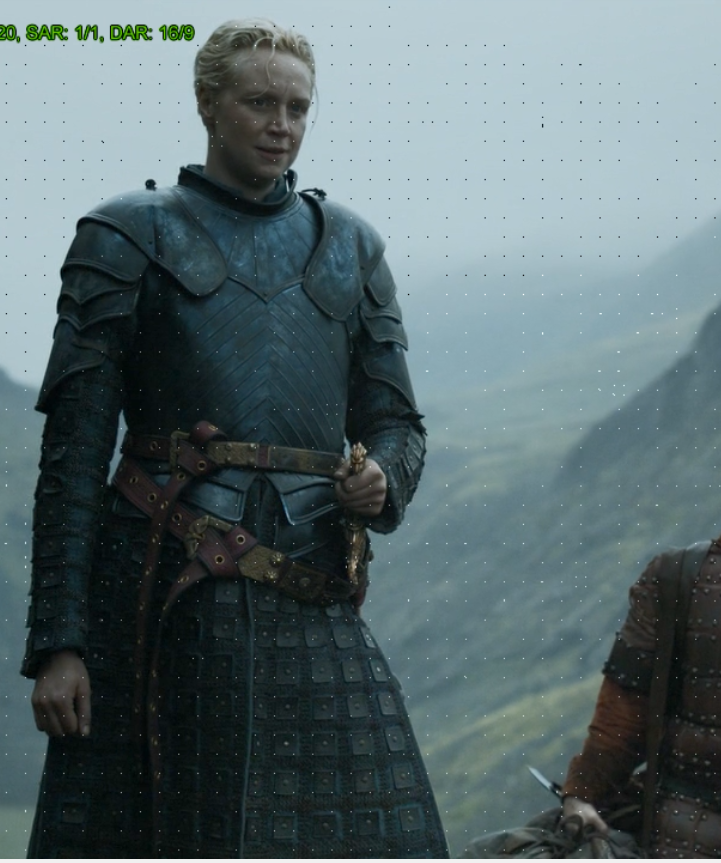
\includegraphics[scale=0.3]{Documeto/1-ElementosTextuais/images/22.png}
    
\includegraphics[scale=0.3]{Documeto/1-ElementosTextuais/images/23.png}

    \small
    Extraído dos vídeos fornecidos pelo Professor
\end{figure}

\subsection{Cenas mais calmas com alta complexidade}
Existem cenas que mesmo que sejam bem lentas, a sua complexidade é muito grande. Isso decorre do fato da complexidade temporal ser baixa, mas da espacial ser grande. No episódio, próximo ao final dele, temos uma cena em uma região montanhosa. Como é de se esperar, essa cena tem bastante textura, muitos detalhes e também camadas. Assim, a sua complexidade espacial é bastante alta.

\begin{figure}[H]
    \centering
    \caption{Imagem do episódio citado de \textit{Game of Trhones}}
    \label{fig:imagem24}
    
    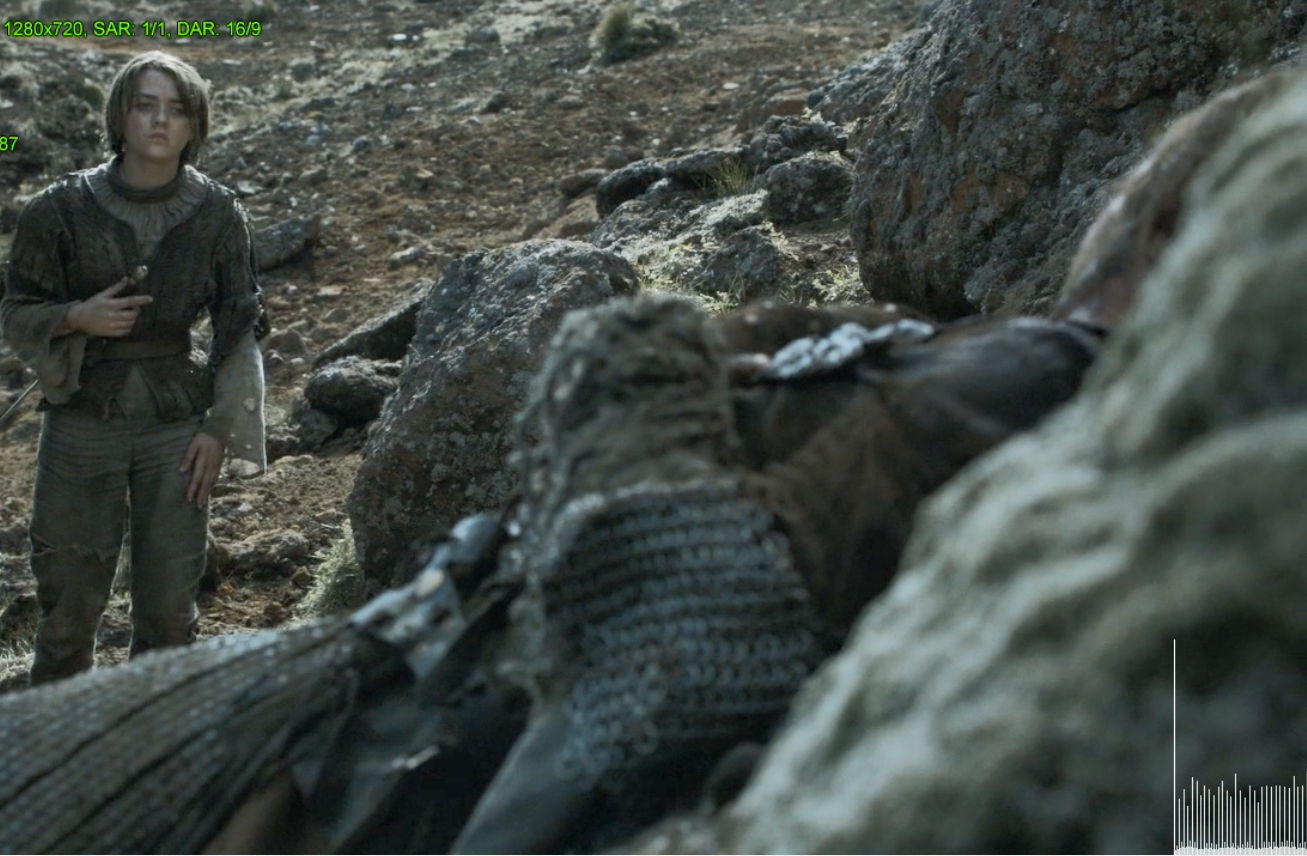
\includegraphics[scale=0.3]{Documeto/1-ElementosTextuais/images/24.png}

    \small
    Extraído dos vídeos fornecidos pelo Professor
\end{figure}
    \captionsetup{justification=centering,margin=0cm}
\label{cap:atividade4}  % Forma de referenciar o capítulo no comando \ref

%inicio do capitulo
\chapter[Atividade 4 - Conversão de vídeo]{Atividade 4 - Conversão de vídeo}

A fim de descobrir as nuances de dois formatos de vídeo x264, x265, AV1 e suas diferenças, a próxima atividade revelará resultados oriundos de uma série de testes para identificar parâmetros para um vídeo considerado bom (transparente) e um ruim (tolerável). Os vídeos utilizados nessa tarefa foram: Big Bunk Bunny e Tears Of Steel.

\section{Atividade 4A - Comprimindo para H.264/AVC}
Irei partir do formato mais antigo e ainda muito utilizado ainda nos dias de hoje, o x264, os resultados serão expostos a seguir.

\paragrafo Big Bunk Bunny: Neste vídeo, iniciei testando o extremo da compressão, gerando um resultado péssimo como esperado. Na tentativa de achar algo transparente, cheguei em 28,5 como fator de qualidade com \textit{bitrate} médio de 1.714Kbps. Enquanto que para algo tolerável, aos olhos bem treinados, a partir de 37, com bitrate médio de 779Kbps. A partir deste ponto o vídeo começa a dar desconforto ao assistir, sendo possível estender até um máximo de 39, que é quando a qualidade fica muito ruim.

\paragrafo Tearls Of Steel: Aqui seguimos a mesma lógica da anterior entretanto o grau de transparência é alcançado até 30, bitrate de 1.623Kbps, e de tolerância em 38, bitrate de 841Kbps, e apesar de possuir um fator maior em comparação ao outro vídeo, no fator máximo ele incomoda consideravelmente mais. 

\paragrafo No geral, a compressão dos vídeos foram rápidas, demorando em média apenas 3 minutos para os vídeos. A Tabela \ref{tab:tabela4a} exibe o Tamanho, bitrate e ratio de cada compressão a fim de melhorar a visualização dos dados.

\begin{table}[H]
    \centering
    \caption{Tabela 4 A}
    \label{tab:tabela4a}
    \begin{tabularx}{\textwidth}{X|C|C|C|C|C|C}
        \hline
        \textbf{Vídeo} & \textbf{Original} & \textbf{Lossless} & \textbf{Lossy} & \textbf{Bitrate Medio (kpbs)} & \textbf{Ratio (original)} & \textbf{Ratio (lossless)} \\ \hline
        Big Buck Bunny (HQ) & 42.462,79 & 10.524,19 & 121,9 & 1714 & 0,00287 & 0,01158 \\ \hline
        Tears Of Steel (HQ) & 44.256,58 & 13.359,21 & 142 & 1623 & 0,00321 & 0,01063 \\ \hline
        Big Buck Bunny (LQ) & 42.462,79 & 10.524,19 & 55,42 & 779 & 0,00131 & 0,01158 \\ \hline
        Tears Of Steel (LQ) & 44.256,58 & 13.359,21 & 73,57 & 841 & 0,00166 & 0,01063 \\ \hline
    \end{tabularx}

    \autoriaPropria
\end{table}


\paragrafo Partindo para uma comparação de eficiência entre CPU e GPU para compressão de vídeo. Na ocasião é uma disputa entre rx580 , que é uma placa gráfica já antiga, e um xeon, que possui muitos núcleos atuando em um programa muito paralelizado, tornando uma disputa relativamente equilibrada. Abaixo a Tabela \ref{tab:tabela4a-continuação} exibe o FPS médio do processo.

\begin{table}[H]
    \centering
    \caption{Tabela 4 A - Continuação}
    \label{tab:tabela4a-continuação}
    \begin{tabularx}{\textwidth}{X|C|C}
        \hline
        \multicolumn{3}{c}{\textbf{FPS}} \\ \hline
        \textbf{Vídeo} & \textbf{h264} & \textbf{VCE h264} \\ \hline
        Tears Of Steel & 107,1 & 124,2 \\ \hline
        Big Buck Bunny & 106,5 & 112,5 \\ \hline
    \end{tabularx}

    \autoriaPropria
\end{table}

\paragrafo Apesar da GPU ter grande vantagem por ser especializada em calculo de matrizes, a CPU possui muitos núcleos para compensar, de maneira a ser muito eficiente para compressão, criando uma diferença consideravelmente pequena entre eles dada sua otimização para tarefa.

\section{Atividade 4B - Comprimindo para H.265/HEVC}
Agora partindo para o próximo formato, o h265. Teoricamente ele possui uma melhor qualidade de compressão, apesar de ser um pouco mais custoso computacionalmente, é isso que iremos observar a partir de agora.

\paragrafo Big Bunk Bunny: Se realmente houveram melhorarias em relação à sua versão an terior, não sabemos dizer só com estes testes, entretanto o formato ainda pesa na compressão, trazendo artefatos e má qualidade com facilidade se não prestar atenção no fator qualidade. Para vídeos transparentes, foi encontrado o fator 26 com \textit{bitrate} de 1708 kbps. Variando um pouco esses parâmetros, obtém-se um vídeo tolerável até o fator 30 com \textit{bitrate} de 1096 kbps; com uma compressão mais abrupta, a qualidade da imagem passa a ser um grande incômodo.

\paragrafo Tearls Of Steel: Aqui serei mais direto, fator qualidade 27,5 para transparente e 32 o tolerável com bitrate de 1596 e 868 respectivamente.

\paragrafo Este formato demorar pouco mais para processar os vídeos, pouco menos de 5 minutos cada, a qualidade é boa com um tamanho/\textit{bitrate} realmente otimizado. As Tabelas \ref{tab:tabela4b} e \ref{tab:tabela4b-continuação} trazem informações detalhadas dos testes, permitindo uma comparação mais específica.

%bunny
%transparente 26
%toleravel 30
%steel
%transparente 27,5
%toleravel 32

\paragrafo 

\begin{table}[H]
    \centering
    \caption{Tabela 4 B}
    \label{tab:tabela4b}
    \begin{tabularx}{\textwidth}{X|C|C|C|C|C|C}
        \hline
        \textbf{Vídeo} & \textbf{Original} & \textbf{Lossless} & \textbf{Lossy} & \textbf{Bitrate Medio (kpbs)} & \textbf{Ratio (original)} & \textbf{Ratio (lossless)} \\ \hline
        Big Buck Bunny (HQ) & 42.462,79 & 10.524,19 & 121,43 & 1708 & 0,00286 & 0,01154 \\ \hline
        Tears Of Steel (HQ) & 44.256,58 & 13.359,21 & 139,67 & 1596 & 0,00316 & 0,01045 \\ \hline
        Big Buck Bunny (LQ) & 42.462,79 & 10.524,19 & 77,94 & 1096 & 0,00184 & 0,00741 \\ \hline
        Tears Of Steel (LQ) & 44.256,58 & 13.359,21 & 75,99 & 868 & 0,00172 & 0,00569 \\ \hline
    \end{tabularx}

    \autoriaPropria
\end{table}

\begin{table}[H]
    \centering
    \caption{Tabela 4 B - Continuação}
    \label{tab:tabela4b-continuação}
    \begin{tabularx}{\textwidth}{X|C|C}
        \hline
        \multicolumn{3}{c}{\textbf{FPS}} \\ \hline
        Vídeo & h265 & VCE h265 \\ \hline
        Tears Of Steel & 63,6 & 121,4 \\ \hline
        Big Buck Bunny & 66,4 & 112,5 \\ \hline
    \end{tabularx}

    \autoriaPropria
\end{table}

\section{Atividade 4C - Comprimindo para AV1}
Finalmente alcançamos o ultimo formato e mais pesado computacionalmente entre eles, trazendo (teoricamente) uma ótima qualidade, afinal, grandes empresas estão por traz dele. Para melhor dinamismo irei apresentar apenas as tabelas e o restante é fácil de explicar.

\begin{table}[H]
    \centering
    \caption{Tabela 4 C}
    \label{tab:tabela4C}
    \begin{tabularx}{\textwidth}{X|C|C|C|C|C|C}
        \hline
        \textbf{Vídeo} & \textbf{Original} & \textbf{Lossless} & \textbf{Lossy} & \textbf{Bitrate Medio (kpbs)} & \textbf{Ratio (original)} & \textbf{Ratio (lossless)} \\ \hline
        Big Buck Bunny (HQ) & 42.462,79 & 10.524,19 & 57,63 & 810 & 0,00136 & 0,00548 \\ \hline
        Tears Of Steel (HQ) & 44.256,58 & 13.359,21 & 128,53 & 1469 & 0,00290 & 0,00962 \\ \hline
        Big Buck Bunny (LQ) & 42.462,79 & 10.524,19 & 26,85 & 378 & 0,00063 & 0,00255 \\ \hline
        Tears Of Steel (LQ) & 44.256,58 & 13.359,21 & 33,08 & 378 & 0,00075 & 0,00248 \\ \hline
    \end{tabularx}

    \autoriaPropria
\end{table}

\begin{table}[H]
    \centering
    \caption{Tabela 4 C - Continuação}
    \label{tab:tabela4c-continuação}
    \begin{tabularx}{\textwidth}{XC}
        \hline
        \multicolumn{2}{c}{\textbf{FPS}} \\ \hline
        Vídeo & VCE AV1 \\ \hline
        Tears Of Steel & 10,9 \\
        Big Buck Bunny & 10,3 \\ \hline
    \end{tabularx}

    \autoriaPropria


\end{table}

\paragrafo Em Big Buck Bunny, o fator de qualidade transparente é 52 e tolerante 63, enquanto para Tears Of Steel os valores são 53 e 63 respectivamente. Quanto a questão do esforço computacional, imaginei que seria demasiado custoso, entretanto não tanto. Um video com Enconder Preset 3, demorou em média 33 minutos para finalizar, enquanto o mesmo com 4 mudou o tempo para 25, o tornando possivelmente inviável para quantidades massivas de vídeos sem uma máquina potente o suficiente ou especializada para a tarefa.


%bunny
%transparente 52
%toleravel 63
%steel
%transparente 53
%toleravel 63

\section{Atividade 4D - Avaliação geral do desempenho dos formatos}
Agora é o momento de comparar os diferentes codecs. Isso é particularmente importante para acompanharmos a evolução dos algoritmos. Todos os arquivos podem ser acessados no link \url{https://drive.google.com/drive/folders/160xDMlNdiJo1Q8intSz2KlbsdiY7OROl}.

\paragrafo O h.264 foi competente em sua função. Apesar da nítida baixa qualidade, o vídeo pode ser assistido sem muitos prejuízos e a sua codificação é bem rápida, se tornando viável para quem não quer muita dor de cabeça com vídeos. No entanto, o h.265 não nos impressionou tanto. Há uma evolução considerável em relação ao h.264, qualidade melhor de imagem, menor presença de artefato, dentre outras vantagens. No entanto, ele deixou a desejar no sentido da velocidade e na taxa de compressão. Pela Tabelas abaixo, podemos observar que a taxa média de compressão foi de, somente, 0,61\%, um resultado quase ínfimo, entretando, inegavelmente com uma qualidade pouco superior.

\paragrafo Em relação ao AV1, esse sim nos impressionou. Se comparado ao h.265 o arquivo também não é tão menor, mas a qualidade da imagem é muito superior. Os artefatos aparecem deforma reduzida e mesmo parâmetros pouco otimizados são suficientes. Digamos que é preciso fazer "muita besteira" para o vídeo ficar ruim.

\paragrafo Nos formatos de vídeo em que se utiliza o hardware, a compressão deixou muito a desejar, demonstrando resultados ruins.


\begin{table}[H]
    \centering
    \caption{Tabela 4 D}
    \label{tab:tabela4d}
    \footnotesize
    \begin{tabularx}{\textwidth}{X|C|C|C|C|C|C|C|C|C}
        \hline
        
        Vídeo & Original & Lossless & Tamanho & Bitrate Medio (kpbs) & Fator de Quali- dade & Velocidade de Compres- são & Ratio (\%) [Arquivo / Original] & Ratio (\%) [Arquivo / Lossless] & Ratio (\%) [Arquivo / h.264] \\ \hline
        Big Buck Bunny h.264HQ & 42.462,79 & 10.524,19 & 121,90 & 1.714,00 & 28,50 & 107,1 & 0,29\% & 1,16\% & - \\ \hline
        Big Buck Bunny h.264LQ & 42.462,79 & 10.524,19 & 55,42 & 779,00 & 37,00 & - & 0,13\% & 0,53\% & - \\ \hline
        Big Buck Bunny h.264 VCE HQ & 42.462,79 & 10.524,19 & 505,00 & 7.104,00 & 28,50 & 124,2 & 1,19\% & 4,80\% & - \\ \hline
        Big Buck Bunny h.265HQ & 42.462,79 & 10.524,19 & 57,63 & 810,00 & 26,00 & 63,60 & 0,14\% & 0,55\% & 0,47 \\ \hline
        Big Buck Bunny h.265LQ & 42.462,79 & 10.524,19 & 26,85 & 378,00 & 30,00 & - & 0,06\% & 0,26\% & 0,48 \\ \hline
        Big Buck Bunny h.265 VCE HQ & 42.462,79 & 10.524,19 & 263,00 & 3.710,00 & 26,00 & 121,40 & 0,62\% & 2,50\% & 0,52 \\ \hline
        Big Buck Bunny AV1 HQ & 42.462,79 & 10.524,19 & 121,43 & 1.708,00 & 52,00 & - & 0,29\% & 1,15\% & 1,00 \\ \hline
        Big Buck Bunny AV1 LQ & 42.462,79 & 10.524,19 & 77,94 & 1.096,00 & 63,00 & - & 0,18\% & 0,74\% & 1,41 \\ \hline
    \end{tabularx}

    \autoriaPropria
\end{table}


\begin{table}[H]
    \centering
    \caption{Tabela 4 D}
    \label{tab:tabela4d}
    \footnotesize
    \begin{tabularx}{\textwidth}{X|C|C|C|C|C|C|C|C|C}
        \hline
        
        Vídeo & Original & Lossless & Tamanho & Bitrate Medio (kpbs) & Fator de Quali- dade & Velocidade de Compres- são & Ratio (\%) [Arquivo / Original] & Ratio (\%) [Arquivo / Lossless] & Ratio (\%) [Arquivo / h.264] \\ \hline
        Tears Of Steel h.264HQ & 44.256,58 & 13.359,21 & 142,00 & 1.623,00 & 30,00 & 106,5 & 0,32\% & 1,06\% & - \\ \hline
        Tears Of Steel h.264LQ & 44.256,58 & 13.359,21 & 73,57 & 841,00 & 38,00 & - & 0,17\% & 0,55\% & - \\ \hline
        Tears Of Steel h.264 VCE HQ & 44.256,58 & 13.359,21 & 389,00 & 4.456,00 & 30,00 & 112,5 & 0,88\% & 2,91\% & - \\ \hline
        Tears Of Steel h.265HQ & 44.256,58 & 13.359,21 & 128,53 & 1.469,00 & 27,50 & 66,40 & 0,29\% & 0,96\% & 1,05 \\ \hline
        Tears Of Steel h.265LQ & 44.256,58 & 13.359,21 & 33,08 & 378,00 & 32,00 & - & 0,07\% & 0,25\% & 0,60 \\ \hline
        Tears Of Steel h.265 VCE HQ & 44.256,58 & 13.359,21 & 275,00 & 3.150,00 & 27,50 & 112,50 & 0,62\% & 2,06\% & 0,54 \\ \hline
        Tears Of Steel AV1 HQ & 44.256,58 & 13.359,21 & 139,67 & 1.596,00 & 53,00 & 10,9 & 0,32\% & 1,05\% & 1,15 \\ \hline
        Tears Of Steel AV1 LQ & 44.256,58 & 13.359,21 & 75,99 & 868,00 & 63,00 & 10,30 & 0,17\% & 0,57\% & 1,37 \\ \hline
    \end{tabularx}


\end{table}
        


    \captionsetup{justification=centering,margin=0cm}
\label{cap:atividade5}  % Forma de referenciar o capítulo no comando \ref

%inicio do capitulo
\chapter[Atividade5: Entendendo, de verdade, o formato JPEG]{Atividade 5: Entendendo, de verdade, o formato JPEG}
O seguinte capítulo tem por objetivo expor as nuances envolvendo o formato JPEG. Para tal, utilizou-se softwares \textit{PackJPG}, \textit{XnView MP} e \textit{RIOT} para coletar diversos dados e, a partir deles, interpretar as suas particularidades.


\begin{table}[H]
    \centering
    \caption{Variação do Tamanho (KB) e o Ratio em função do Fator de Qualidade e \textit{Subsampling}.}
    \label{tab:6a}

    \scriptsize
    \begin{tabularx}{\textwidth}{X|C|C|C|C|C|C|C|C|C|C|C}
    \hline
        \multirow{2}{*}{\textbf{Imagem}} & \multirow{2}{*}{\textbf{\makecell{Fator\\Qual.}}} & \multicolumn{5}{c|}{\textbf{Tamanhos (KB)}} & \multicolumn{5}{c}{\textbf{Ratios (\%)}} \\ \hhline{~~----------}
        ~ & ~ & \textbf{4:4:4} & \textbf{4:2:2} & \textbf{4:2:0} & \textbf{4:1:1} & \textbf{4:0:0*} & \textbf{4:4:4} & \textbf{4:2:2} & \textbf{4:2:0} & \textbf{4:1:1} & \textbf{4:0:0*} \\ \hline
        48 & 30 & 242,55 & 208,2 & 247,7 & 187,69 & 162,55 & 5,75\% & 4,93\% & 5,87\% & 4,45\% & 3,85\% \\ \hline
        46 & 60 & 214,8 & 182,11 & 163,83 & 162,97 & 137,1 & 5,09\% & 4,32\% & 3,88\% & 3,86\% & 3,25\% \\ \hline
        39 & 55 & 238,29 & 203,92 & 184 & 184,05 & 158,95 & 5,65\% & 4,83\% & 4,36\% & 4,36\% & 3,77\% \\ \hline
        35 & 55 & 182,68 & 153,78 & 136,88 & 136,72 & 113,28 & 4,33\% & 3,64\% & 3,24\% & 3,24\% & 2,68\% \\ \hline
        33 & 60 & 367,75 & 267,56 & 215,85 & 212,3 & 160,75 & 8,72\% & 6,34\% & 5,12\% & 5,03\% & 3,81\% \\ \hline
        18 & 55 & 124,72 & 103,87 & 87,96 & 89,83 & 64,98 & 2,96\% & 2,46\% & 2,08\% & 2,13\% & 1,54\% \\ \hline
        16 & 60 & 184,25 & 153,51 & 133,73 & 135,53 & 107,03 & 4,37\% & 3,64\% & 3,17\% & 3,21\% & 2,54\% \\ \hline
        3 & 95 & 154,54 & 139,19 & 131,68 & 132,07 & 124,38 & 3,66\% & 3,30\% & 3,12\% & 3,13\% & 2,95\% \\ \hline 
    \end{tabularx}

    \autoriaPropria

\end{table}

\paragrafo As diferenças entre diferentes técnicas de chroma subsampling mostraram-se, na maioria dos testes, visualmente irrelevantes. Isso ocorre porque essa técnica remove informações de crominância, que nossos olhos geralmente não percebem. Portanto, desde que não haja macro blocos visíveis, os diferentes métodos utilizados(4.2.2, 4.2.0 ou 4.1.1) não introduzem mudanças visíveis ou perda significativa de detalhes (pelo menos foi o que observei). Em muitos casos, pode-se optar pelo método mais leve sem comprometer muito a qualidade da imagem. No entanto, ainda persiste a questão sobre por que o chroma subsampling mais comum é o 4:4:0.

\paragrafo Em relação aos testes realizados, houve uma exceção notável. Na imagem 33, houve uma deterioração drástica na qualidade, independentemente do método de subsampling utilizado. Isso sugere que os métodos de subsampling mais leves podem não ser adequados para imagens com alto conteúdo de pequenas partículas coloridas ou macro blocos visíveis, como testei com a imagem 33, imagem com folhas de árvores laranjas. No entanto, é importante ressaltar que esses casos são menos comuns e que, para a maioria das imagens, é possível manter uma boa qualidade com métodos de subsampling mais leves.

\paragrafo Quanto à escala de cinza, achei-a bastante interessante. No entanto, ao optar pela escala grayscale, a escolha não é mais ditada pela compressão, mas sim por considerações estéticas. A menos que haja uma necessidade extrema de compressão, não vejo motivo prático para utilizar a escala de cinza em detrimento da qualidade de imagem.

\begin{table}[H]
    \centering
    \caption{Avaliação dos Artefatos do JPEG}
    \label{tab:6b}

    \footnotesize
    \begin{tabularx}{\textwidth}{X|C|C|C|C}
    \hline
        \textbf{Imagem} & \textbf{Pontos} & \textbf{Fator Qual.} & \textbf{Tamanho (KB)} & \textbf{\textit{Ratio} (\%)} \\ \hline
        \multirow{4}{*}{48} & Transparência & 40 & 254,09 & 6,02\% \\ \hhline{~----}
        ~ & Ruídos de Mosquito & 5 & 45,38 & 1,08\% \\ \hhline{~----}
        ~ & Macroblocos Visíveis & 5 & 45,38 & 1,08\% \\ \hhline{~----}
        ~ & Baixa Qualidade & 5 & 45,38 & 1,08\% \\ \hline
        \multirow{4}{*}{46} & Transparência & 55 & 154,39 & 3,66\% \\ \hhline{~----}
        ~ & Ruídos de Mosquito & 35 & 119,12 & 2,82\% \\ \hhline{~----}
        ~ & Macroblocos Visíveis & 15 & 65,12 & 1,54\% \\ \hhline{~----}
        ~ & Baixa Qualidade & 15 & 65,12 & 1,54\% \\ \hline
        \multirow{4}{*}{39} & Transparência & 55 & 202 & 4,79\% \\ \hhline{~----}
        ~ & Ruídos de Mosquito & 35 & 139,52 & 3,31\% \\ \hhline{~----}
        ~ & Macroblocos Visíveis & 30 & 122,01 & 2,89\% \\ \hhline{~----}
        ~ & Baixa Qualidade & 10 & 43,82 & 1,04\% \\ \hline
        \multirow{4}{*}{35} & Transparência & 55 & 153,78 & 3,64\% \\ \hhline{~----}
        ~ & Ruídos de Mosquito & 35 & 107,61 & 2,55\% \\ \hhline{~----}
        ~ & Macroblocos Visíveis & 25 & 82,37 & 1,95\% \\ \hhline{~----}
        ~ & Baixa Qualidade & 10 & 37,43 & 0,89\% \\ \hline
        \multirow{4}{*}{33} & Transparência & 45 & 205,86 & 4,88\% \\ \hhline{~----}
        ~ & Ruídos de Mosquito & 20 & 96,83 & 2,30\% \\ \hhline{~----}
        ~ & Macroblocos Visíveis & 15 & 71,05 & 1,68\% \\ \hhline{~----}
        ~ & Baixa Qualidade & 10 & 43,86 & 1,04\% \\ \hline
        \multirow{4}{*}{18} & Transparência & 50 & 94,98 & 2,25\% \\ \hhline{~----}
        ~ & Ruídos de Mosquito & 35 & 73,38 & 1,74\% \\ \hhline{~----}
        ~ & Macroblocos Visíveis & 25 & 56,98 & 1,35\% \\ \hhline{~----}
        ~ & Baixa Qualidade & 5 & 17,63 & 0,42\% \\ \hline
        \multirow{4}{*}{16} & Transparência & 40 & 129,52 & 3,07\% \\ \hhline{~----}
        ~ & Ruídos de Mosquito & 25 & 88,36 & 2,09\% \\ \hhline{~----}
        ~ & Macroblocos Visíveis & 15 & 57,66 & 1,37\% \\ \hhline{~----}
        ~ & Baixa Qualidade & 8 & 31,83 & 0,75\% \\ \hline
        \multirow{4}{*}{3} & Transparência & 75 & 54,19 & 1,28\% \\ \hhline{~----}
        ~ & Ruídos de Mosquito & 50 & 34,76 & 0,82\% \\ \hhline{~----}
        ~ & Macroblocos Visíveis & 50 & 34,76 & 0,82\% \\ \hhline{~----}
        ~ & Baixa Qualidade & 25 & 21,66 & 0,51\% \\ \hline
    \end{tabularx}

    \autoriaPropria

\end{table}

\paragrafo De acordo com os nossos testes, os artefatos visuais são relativos ao conteúdo da imagem, variando conforme bordas definidas, excesso de partículas, degradês, entre outros. As características das imagens influenciam significativamente na percepção da qualidade após a aplicação do chroma subsampling, que é um método de compressão com perdas.

\paragrafo Em imagens com degradês, há a tendência de surgir camadas perceptíveis (macro blocos), enquanto em imagens com bordas bem definidas, é comum aparecer ruído de mosquito, onde um pode aparecer antes do outro a depender destes detalhes. Quando há muitas partículas ou macroblocos visíveis, o subsampling pode causar alterações notáveis. Isso na prática foi bem simples ver alterações na imagem 3, entretanto na imagem 48 já tive mais dificuldade, onde inicialmente não percebi o ajuste de foco. Apenas ao revisitar a imagem notei essa diferença.

\paragrafo Também é importante ressaltar que a aplicação de chroma subsampling pode causar uma variação visível mesmo com o fato qualidade máximo na conversão do arquivo (Principalmente com o JPEG, formato utilizado nesta atividade), ocasionando compressões de baixa qualidade independnete do fator citado.

\paragrafo O próximo teste consiste em verificar a eficácia de compressão de diferentes algoritmos em imagens JPEG. A Tabela \ref{tab:6c}.
\begin{table}[H]
    \centering
    \caption{Recomprindo o JPEG}
    \label{tab:6c}

    \footnotesize
    \begin{tabularx}{\textwidth}{X|C|C|C|C|C|C}
    
    \hline
    \multirow{2}{*}{\makecell{\textbf{JPEG}\\\textbf{Original}\\\textbf{(bytes)}}} & \multicolumn{2}{c|}{\textbf{Pack RAR}} & \multicolumn{2}{c|}{\textbf{Pack ZIP}} \multicolumn{2}{c}{\textbf{wxPackJPG}} \\ \hhline{~------}
    ~ & \textbf{Tamanho (bytes)}	& \textbf{Ratio (\%)} & \textbf{Tamanho (bytes)} &	\textbf{Ratio (\%)}	& \textbf{Tamanho (bytes)} &	\textbf{Ratio (\%)} \\\hline
    11 & 11 & 99,12\% & 11,3 & 99,12\% & 9 & 80,09\% \\ \hline

    \end{tabularx}

    \autoriaPropria

\end{table}

\paragrafo Como pode-se observar, o RAR e ZIP quase não conseguiram comprimir mais os arquivos. Assim, não faz sentido comprimir esses arquivos em RAR ou ZIP, visto que não foram projetados para compressão de imagens, especificamente. No entanto, o \textit{wxPackJPG} obteve um ratio de 80\%, uma quantidade certamente considerável. Isso ocorre, pois diferente do RAR e do ZIP, que tentam encontrar relações entre os \textit{pixels} linha a linha, o \textit{wxPackJPG} divide a imagens em blocos e busca a melhor forma de compressão para cada um deles, seja leitura dos \textit{pixels} linha a linha, coluna a coluna ou em zig-zag na diagonal. Assim, ele utiliza o melhor método de compressão para cada caso.

\paragrafo Assim, o \textit{wxPackJPG} torna-se extremamente útil caso tenha um método fácil de exibi-lo via qualquer software e seria maravilhoso utiliza-lo para web. Além disso, backups também podem se beneficiar desses métodos. Entretanto, por uma diminuição de 20\% não penso que seria um real sucessor do JPEG, o qual está muito consolidado na internet atualmente.
    \include{Documeto/1-ElementosTextuais/1-Desenvolvimento/6-atividade6}
    \captionsetup{justification=centering,margin=0cm}
\label{cap:atividade7}  % Forma de referenciar o capítulo no comando \ref

%inicio do capitulo
\chapter[Atividade7: Otimizando imagens]{Atividade 7: Otimizando imagens}
Será que já exploramos todas as formas de compressão e otimização possíveis? Giraldeli acredita que não. Por isso, vamos analisar e discutir o software PINGO e sua interface gráfica, PINGA, desenvolvida pelo próprio criador.
Na imagem abaixo, é possível observar as taxas médias de compressão, tanto em modos lossless quanto "lossy"/Near-lossless (explicaremos isso em breve), a partir de imagens PNG-24 adquiridas das imagens originais.

\begin{table}[H]
\centering
\caption{Otimização de imagens em PNG}
\begin{tabularx}{\textwidth}{X|C|C|C|C}
\hline
\multirow{2}{*}{\textbf{\makecell[c]{PNG Original\\(bytes)}}} & \multicolumn{2}{c|}{\textbf{\textit{Lossless}}} & \multicolumn{2}{c}{\textbf{\textit{Near-Lossless}}} \\ \hhline{~----}
~ & Tamanho (bytes) & Ratio (\%) & Tamanho (bytes) & Ratio (\%) \\ \hline

113.944.706 & 109.971.161 & 96,51\% & 46.038.976 & 40,40\% \\
\hline
\end{tabularx}

\autoriaPropria
\end{table}

\paragrafo De início, percebe-se que o formato lossless não oferece uma redução significativa. No entanto, o modo Near-lossless surgiu como uma solução promissora e interessante.

\paragrafo O formato Near-lossless é um método de compressão com perdas (lossy) que visa otimizar outros formatos de compressão. Nesse formato, pequenas variações pontuais que dificultariam a compressão lossless são eliminadas. Por exemplo, em uma imagem de um céu limpo, pode haver várias tonalidades de azul. O Near-lossless "padroniza" essas tonalidades (sem que haja mudanças visíveis) para que, após a aplicação de uma compressão realmente lossless, a eficiência seja muito maior.

\paragrafo A tabela a seguir apresenta dados relativos à compressão Near-lossless utilizada.

\begin{table}[H]
    \centering
    \caption{Avaliação dos Artefatos do JPEG}
    \label{tab:6b}

    \footnotesize
    \begin{tabularx}{\textwidth}{X|C|C|C}
    \hline
        Descrição & Tamanho PNG Original & Tamanho PNG Near-lossless & Redução (\%) \\ \hline
        IMG01 & 1.613.669 & 470.751 & 70,8\% \\ 
        IMG02 & 2.126.163 & 744.135 & 65,0\% \\ 
        IMG03 & 1.042.306 & 276.561 & 73,5\% \\ 
        IMG04 & 1.822.802 & 586.640 & 67,8\% \\ 
        IMG05 & 1.885.248 & 517.736 & 72,5\% \\ 
        IMG06 & 1.915.684 & 707.084 & 63,1\% \\ 
        IMG07 & 1.572.060 & 445.175 & 71,7\% \\ 
        IMG08 & 3.513.270 & 1.988.475 & 43,4\% \\ 
        IMG09 & 1.960.195 & 589.413 & 69,9\% \\ 
        IMG10 & 2.509.826 & 889.026 & 64,6\% \\ 
        IMG11 & 3.224.670 & 1.472.274 & 54,3\% \\ 
        IMG12 & 2.569.986 & 1.014.155 & 60,5\% \\ 
        IMG13 & 2.568.571 & 965.602 & 62,4\% \\ 
        IMG14 & 2.329.559 & 934.462 & 59,9\% \\ 
        IMG15 & 1.156.266 & 250.572 & 78,3\% \\ 
        IMG16 & 2.489.280 & 1.006.796 & 59,6\% \\ 
        IMG17 & 2.466.793 & 921.658 & 62,6\% \\ 
        IMG18 & 1.906.284 & 616.201 & 67,7\% \\ 
        IMG19 & 2.683.151 & 1.079.954 & 59,8\% \\ 
        IMG20 & 3.127.814 & 1.648.449 & 47,3\% \\ 
        IMG21 & 1.582.110 & 596.268 & 62,3\% \\ 
        IMG22 & 2.649.058 & 1.113.681 & 58,0\% \\ 
        IMG23 & 2.246.862 & 930.639 & 58,6\% \\ 
        IMG24 & 2.412.455 & 1.250.916 & 48,1\% \\ 
        IMG25 & 2.287.870 & 838.609 & 63,3\% \\ 
        IMG26 & 1.676.966 & 568.036 & 66,1\% \\ 
        IMG27 & 3.220.560 & 1.526.112 & 52,6\% \\ 
        IMG28 & 2.325.051 & 1.089.100 & 53,2\% \\ 
        IMG29 & 692.210 & 244.930 & 64,6\% \\ 
        IMG30 & 1.445.622 & 338.954 & 76,6\% \\ 
        IMG31 & 1.881.345 & 905.145 & 51,9\% \\ 
        IMG32 & 2.533.661 & 925.294 & 63,5\% \\ 
        IMG33 & 2.956.042 & 1.499.003 & 49,3\% \\ 
        IMG34 & 2.046.515 & 534.616 & 73,9\% \\ 
        IMG35 & 2.304.984 & 904.325 & 60,8\% \\ 
        IMG36 & 1.092.302 & 390.488 & 64,3\% \\ 
        IMG37 & 2.822.178 & 1.121.492 & 60,3\% \\ 
        IMG38 & 3.048.615 & 1.410.537 & 53,7\% \\ 
        IMG39 & 2.564.862 & 1.133.122 & 55,8\% \\ 
        IMG40 & 2.384.943 & 826.070 & 65,4\% \\ 
        IMG41 & 3.048.024 & 1.488.942 & 51,2\% \\ 
        IMG42 & 1.187.267 & 311.156 & 73,8\% \\ 
        IMG43 & 2.814.564 & 1.300.451 & 53,8\% \\ 
        IMG44 & 3.201.971 & 1.568.705 & 51,0\% \\ 
        IMG45 & 2.506.005 & 1.117.689 & 55,4\% \\ 
        IMG46 & 2.332.555 & 902.688 & 61,3\% \\ 
        IMG47 & 2.309.341 & 778.783 & 66,3\% \\ 
        IMG48 & 3.387.244 & 1.815.708 & 46,4\% \\ 
        IMG49 & 2.044.998 & 536.091 & 73,8\% \\ 
        IMG50 & 2.454.929 & 946.307 & 61,5\% \\ \hline
        \textit{MÍNIMO} & 692.210 & 244.930 & 43,4\% \\ 
        \textit{MÉDIO} & 2.278.894 & 920.780 & 61,4\% \\ 
        \textit{MÁXIMO} & 3.513.270 & 1.988.475 & 78,3\% \\ 
    \end{tabularx}

    \autoriaPropria
\end{table}

\paragrafo com estes dados, é possível observar que as melhores compressões ocorrem em imagens com poucas cores ou com grandes áreas monocromáticas, como nas imagens 1, 3, 5, 7, 15, 30, 34 e 42, onde todas apresentam mais de 70\% de redução.

\paragrafo Num geral, as imagens geradas são fascinantes\footnote{Durante as comparações das imagens, fiquei muito tempo analizando se as cores das imagens estavam diferentes ou se era loucura da minha cabeça kk}, é em sua grande maioria transparente a imagem original e é enormemente mais eficiente (em bytes), se levarmos em consideração o fato de ser "lossless".

\paragrafo Abaixo estão são demonstrados uma comparação antes e depois da compressão nas imagens 11 e 15.

\includegraphics[scale=0.24]{Documeto/1-ElementosTextuais/1-Desenvolvimento/Imagens-atividade7/IMG11.png}

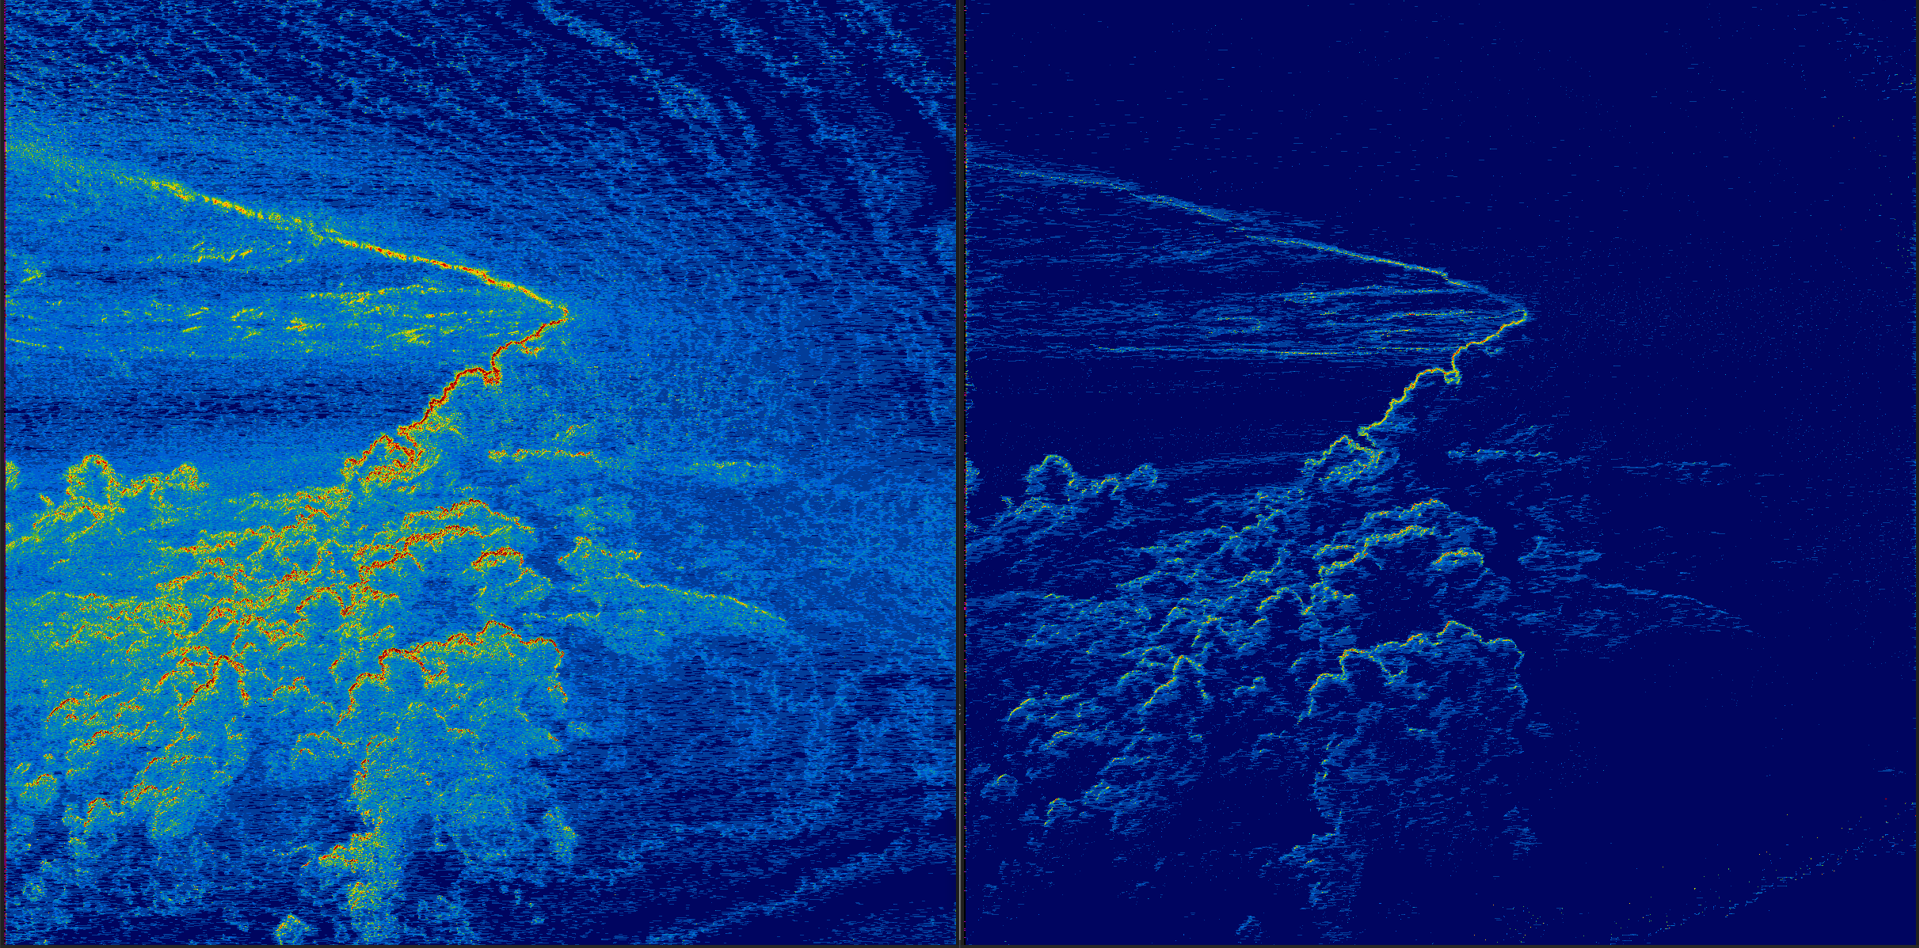
\includegraphics[scale=0.24]{Documeto/1-ElementosTextuais/1-Desenvolvimento/Imagens-atividade7/IMG15.png}

\paragrafo Vale ressaltar também a tabela de relação entre cor e quantidade de bits utilizados, imagem, retirada dos slides da matéria, abaixo:

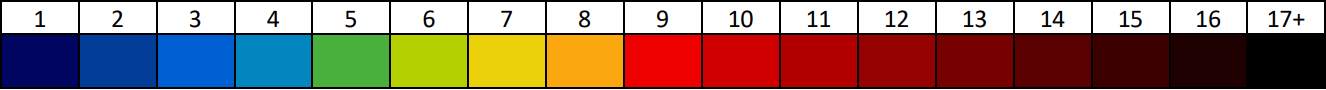
\includegraphics[scale=0.35]{Documeto/1-ElementosTextuais/1-Desenvolvimento/Imagens-atividade7/Tabela.png}


\paragrafo Com base nas imagens, observamos que há uma redução expressiva de complexidade entre elas, resultando em um arquivo .png muito mais otimizado.\footnote{A diferença de coloração da imagem utilizando o pngthermal é bizarroooo}

\paragrafo Entretanto, como nem tudo são flores, houve exceções que, após a aplicação do método supracitado, apresentaram mudanças visíveis. Começando pelas diferenças menores:

Observamos que nas imagens 21 e 44, o céu apresentava vários pontos espalhados (apesar de ser necessário dar zoom para observá-los com clareza).
Na imagem 5, há uma mudança imperceptível sem a presença da imagem original. Na água, há ladrilhos que são mais visíveis na imagem original, enquanto na imagem com a técnica aplicada, eles ficam opacos.
Na imagem 39, há uma camada no céu.
Finalmente, as falhas mais visíveis, sendo possível observá-las facilmente, estão nas imagens 15 e 29. Ambas apresentam macroblocos visíveis. Na imagem 29, pequenos macroblocos aparecem na parte inferior direita da flor. Entretanto e Surpreendentemente, a imagem 15, que apresentou o melhor percentual de compressão, também apresentou a pior compressão em termos visuais, com macroblocos muito visíveis facilmente no canto inferior direito da imagem.

\paragrafo De modo geral, o software apresentado demonstrou ser extremamente útil e eficiente, alcançando uma taxa média de compressão (ratio) de 38,6 a partir da imagem original. Isso o torna uma opção viável para armazenar um grande volume de fotos, especialmente para fins de recordação e em situações em que a qualidade da imagem é mais importante do que a otimização.

\paragrafo Desta forma, também é interessante buscarmos melhores compressões para aqueles que priorizam maiores otimizações, mantendo a qualidade das imagens. Vamos abordar a compressão Lossy, utilizando um software que compara a imagem original com várias versões dela, cada uma com um fator Q diferente, permitindo ajustar o parâmetro de mudança média. Ficou confuso? Vou explicar melhor.

\paragrafo Abaixo, apresentamos a redução em \% das compressões realizadas, utilizando o padrão do software. A "Redução JPEG Câmera" refere-se à redução adicional feita sobre a compressão realizada pela própria câmera.

\begin{table}[H]
    \centering
    \caption{Otimizando Imagens em JPEG (Modo Lossy, em KB)}
    \label{tab:6b}

    \footnotesize
    \begin{tabularx}{\textwidth}{X|C|C|C|C|C}
    \hline
        Imagem & Tam Sem Compressão & Tam. JPEG Câmera & Ratio JPEG Câmera (\%) & Tam. JPEG Otimizado & \% Redução JPEG Câmera \\ \hline
        IMG01 & 26.791 & 2.278 & 8,5\% & 1199 & 47,4\% \\ 
        IMG02 & 26.791 & 1.777 & 6,6\% & 814 & 54,2\% \\ 
        IMG03 & 26.791 & 3.151 & 11,8\% & 1710 & 45,7\% \\ 
        IMG04 & 26.791 & 2.512 & 9,4\% & 1244 & 50,5\% \\ 
        IMG05 & 26.791 & 7.918 & 29,6\% & 718 & 90,9\% \\ 
        IMG06 & 26.791 & 1.814 & 6,8\% & 1438 & 20,7\% \\ 
        IMG07 & 26.791 & 2.113 & 7,9\% & 1009 & 52,2\% \\ 
        IMG08 & 26.791 & 3.977 & 14,8\% & 2115 & 46,8\% \\ 
        IMG09 & 26.791 & 2.312 & 8,6\% & 1578 & 31,7\% \\ 
        IMG10 & 26.791 & 2.100 & 7,8\% & 1381 & 34,2\% \\ 
        IMG11 & 26.791 & 5.724 & 21,4\% & 3373 & 41,1\% \\ 
        IMG12 & 26.791 & 2.409 & 9,0\% & 1290 & 46,5\% \\ 
        IMG13 & 26.791 & 5.227 & 19,5\% & 2966 & 43,3\% \\ 
        IMG14 & 26.791 & 2.733 & 10,2\% & 1524 & 44,2\% \\ 
        IMG15 & 26.791 & 4.460 & 16,6\% & 2745 & 38,5\% \\ 
        IMG16 & 26.791 & 3.646 & 13,6\% & 1878 & 48,5\% \\ 
        IMG17 & 26.791 & 2.386 & 8,9\% & 1353 & 43,3\% \\ 
        IMG18 & 26.791 & 1.156 & 4,3\% & 696 & 39,8\% \\ 
        IMG19 & 26.791 & 1.561 & 5,8\% & 1113 & 28,7\% \\ 
        IMG20 & 26.791 & 5.005 & 18,7\% & 2897 & 42,1\% \\ \hline
        \textbf{MÍNIMO} & 26.791 & 1.156 & 4,3\% & 696 & 20,7\% \\ 
        \textbf{MÉDIO} & 26.791 & 3.213 & 11,99\% & 1.652 & 44,5\% \\ 
        \textbf{MÁXIMO} & 26.791 & 7.918 & 29,6\% & 3.373 & 90,9\% \\ 
    \end{tabularx}

    \autoriaPropria
\end{table}

\paragrafo Pode-se observar que já alcançamos uma boa otimização, mas, surpreendentemente, o fator de qualidade está no nível mais alto, preservando o máximo de qualidade, embora menos otimizado. Observando as imagens lado a lado ou sequencialmente, todas parecem absolutamente idênticas nos testes realizados. Contudo, não paramos por aí. Decidi testar a compressão no índice mínimo de fidelidade, mesmo que isso impactasse a transparência das imagens. Os dados e imagens dos resultados serão mostrados a seguir.

\begin{table}[H]
    \centering
    \caption{Otimizando Imagens em JPEG LOW(Modo Lossy, em KB)}
    \label{tab:6b}

    \footnotesize
    \begin{tabularx}{\textwidth}{X|C|C|C|C|C}
    \hline
        Imagem & Tam Sem Compressão & Tam. JPEG Câmera & Ratio JPEG Câmera (\%) & Tam. JPEG Otimizado (low)\textbf{} & \% Redução JPEG Câmera \\ \hline 
        IMG01 & 26.791 & 2.278 & 8,5\% & 537 & 76,4\% \\ 
        IMG02 & 26.791 & 1.777 & 6,6\% & 278 & 84,4\% \\ 
        IMG03 & 26.791 & 3.151 & 11,8\% & 666 & 78,9\% \\ 
        IMG04 & 26.791 & 2.512 & 9,4\% & 476 & 81,1\% \\ 
        IMG05 & 26.791 & 7.918 & 29,6\% & 251 & 96,8\% \\ 
        IMG06 & 26.791 & 1.814 & 6,8\% & 356 & 80,4\% \\ 
        IMG07 & 26.791 & 2.113 & 7,9\% & 378 & 82,1\% \\ 
        IMG08 & 26.791 & 3.977 & 14,8\% & 732 & 81,6\% \\ 
        IMG09 & 26.791 & 2.312 & 8,6\% & 473 & 79,5\% \\ 
        IMG10 & 26.791 & 2.100 & 7,8\% & 434 & 79,3\% \\ 
        IMG11 & 26.791 & 5.724 & 21,4\% & 1344 & 76,5\% \\ 
        IMG12 & 26.791 & 2.409 & 9,0\% & 535 & 77,8\% \\ 
        IMG13 & 26.791 & 5.227 & 19,5\% & 1088 & 79,2\% \\ 
        IMG14 & 26.791 & 2.733 & 10,2\% & 584 & 78,6\% \\ 
        IMG15 & 26.791 & 4.460 & 16,6\% & 1153 & 74,1\% \\ 
        IMG16 & 26.791 & 3.646 & 13,6\% & 658 & 82,0\% \\ 
        IMG17 & 26.791 & 2.386 & 8,9\% & 556 & 76,7\% \\ 
        IMG18 & 26.791 & 1.156 & 4,3\% & 323 & 72,1\% \\ 
        IMG19 & 26.791 & 1.561 & 5,8\% & 191 & 87,8\% \\ 
        IMG20 & 26.791 & 5.005 & 18,7\% & 1050 & 79,0\% \\ \hline
        \textbf{MÍNIMO} & 26.791 & 1.156 & 4,3\% & 191 & 72,1\% \\ 
        \textbf{MÉDIO} & 26.791 & 3.213 & 11,99\% & 603 & 80,2\% \\ 
        \textbf{MÁXIMO} & 26.791 & 7.918 & 29,6\% & 1.344 & 96,8\% \\ 
    \end{tabularx}

    \autoriaPropria
\end{table}

\paragrafo Nos testes realizados com a resolução no nível mais baixo (maior otimização), nem todas as imagens mantêm a transparência perfeita. No entanto, as mudanças são mínimas, tornando viável, em nossa opinião, o uso consistente desse método. As únicas alterações perceptíveis ocorreram nas sombras das imagens 1, 2, 3, 4, 12\footnote{Durante a realização dos testes, ficávamos alternando entre as imagens em tela cheia no monitor, e na imagem 12, teve uma situação engraçada, nela parecia ter uma espécie de sobrancelha subindo e descendo conforme alternavamos entre as imagens}, 15, 16 e 17, de forma trivial. Portanto, quando se trata de otimização de imagens com foco em maior compressão, este método é extremamente eficiente.

    \captionsetup{justification=centering,margin=0cm}
\label{cap:atividade8}  % Forma de referenciar o capítulo no comando \ref

%inicio do capitulo
\chapter[Atividade8: Avaliando os candidatos a sucessor do JPEG]{Atividade 8: Avaliando os candidatos a sucessor do JPEG}

Tá, mas e o sucessor do JPEG? Um bom velho de guerra que já está na internet há muitos anos, mas cuja a tecnologia já é defasada. Uma série de outros formatos melhores tecnicamente surgiram, então vamos analisar esses formatos e seus comportamentos.

\paragrafo Primeiramente, vamos comparar o \textit{ratio} de diferentes formatos. A Tabela abaixo traz essa métrica em três formatos diferentes, WEBP, JPEG XL e AVIf. Dentre eles, o AVIF foi o que teve melhor taxa de compressão, no entanto sua compressão é bem mais pesada que os demais. Ele demorou quase uns dois minutos, enquanto o JEPG XL\footnote{Para a Geração Z uma eternidade.} comprimiu em apenas uns 30 segundos. Dentre eles, o JPEG XL pareceu-me o ideal, chegou muito perto da compressão do AVIF com um pouco mais de tempo do que se comparado ao WEBP.

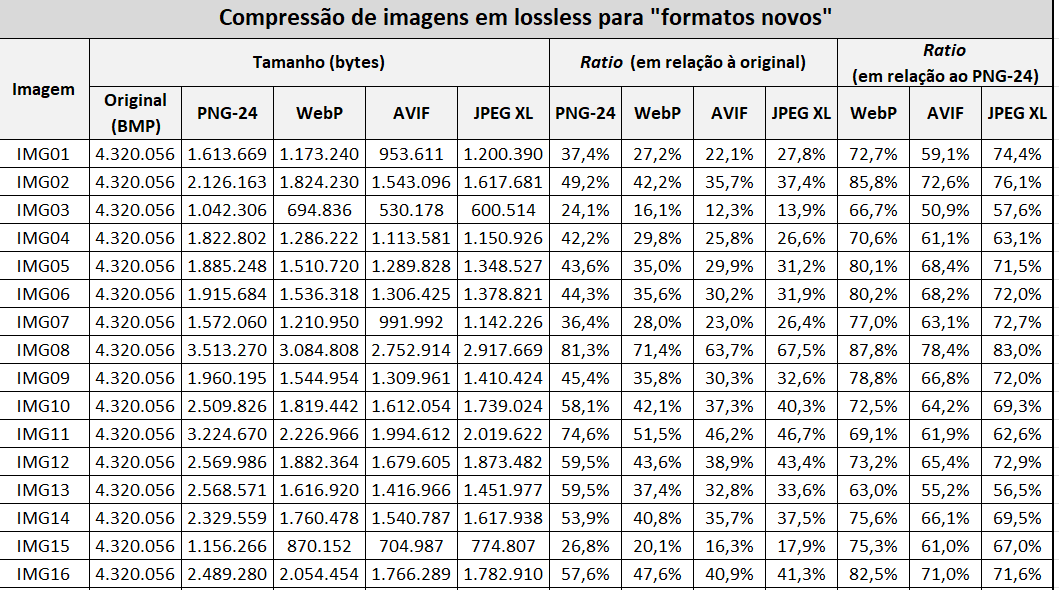
\includegraphics[scale=0.6]{Documeto/1-ElementosTextuais/1-Desenvolvimento/2.png}

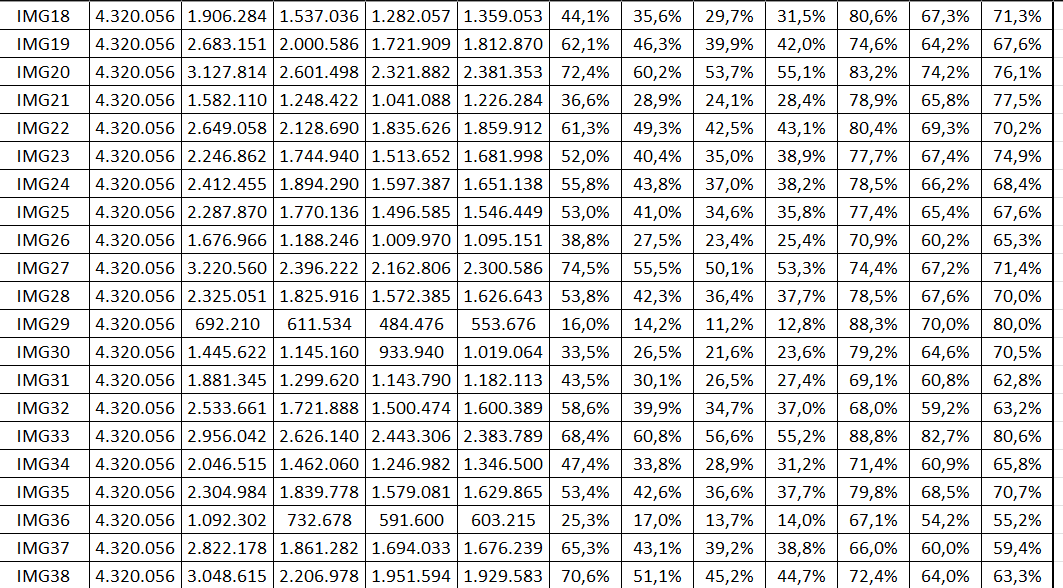
\includegraphics[scale=0.6]{Documeto/1-ElementosTextuais/1-Desenvolvimento/3.png}

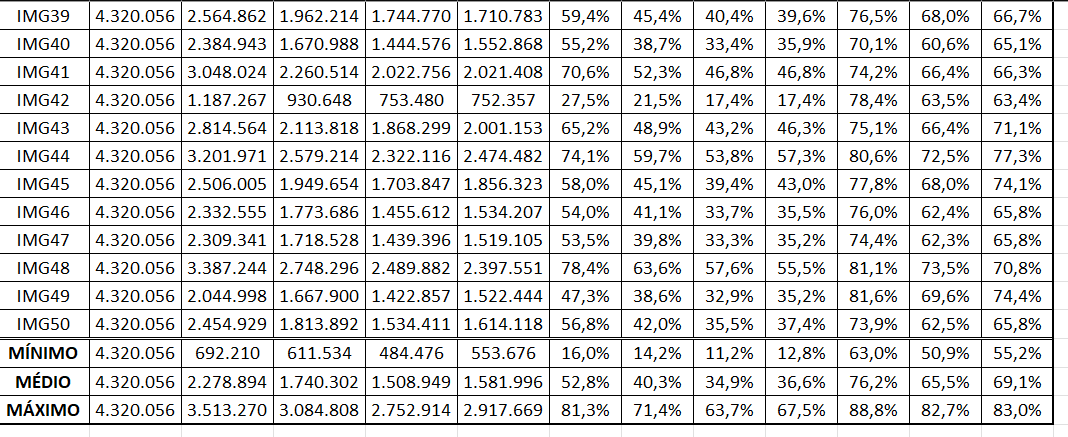
\includegraphics[scale=0.6]{Documeto/1-ElementosTextuais/1-Desenvolvimento/4.png}

\paragrafo  Agora, tem-se a \ref{tab:8b}, que busca comparar diferentes formatos mais hodiernos. Pelas nossas observações, o AVIF acabou por ser o mais indicado se o fator compressão é o mais importante. A sua compressão é muito boa, chegando a resultados surpreendentes; no entanto, seu "peso" acaba por ser muito ruim em alguns momentos. A sua compressão é bastante demorada, não sendo um impeditivo, mas uma desvantagem. Em contra partida, o JPEGXL apresentou taxas de compressão menores, mas bem mais rápidas.

\begin{table}[H]
\centering
\caption{Compressão de imagens em lossy para "formatos novos"
(Qualidade Transparente)}
\label{8b}
\begin{tabularx}{\textwidth}{X|C|C|C|C|C|C|C|C|C}
\hline
 Tamanho (bytes) & ~ & ~ & ~ & ~ & Fator de Qualidade & ~ & ~ & ~ \\ \hline
        IMAGEM & Original (BMP) & JPEG & WebP & HEIC & JPEG XL & JPEG & WebP & HEIC & JPEG XL \\ \hline
        48 & 4.320.056 & 254.090 & 310.686 & 340.733 & 188.416 & 40 & 29 & 42 & 48 \\ \hline
        46 & 4.320.056 & 154.390 & 114.576 & 93.146 & 163.148 & 55 & 45 & 40 & 61 \\ \hline
        39 & 4.320.056 & 202.000 & 183.898 & 781.926 & 104.703 & 55 & 37 & 46 & 65 \\ \hline
        35 & 4.320.056 & 153.780 & 107.850 & 331.787 & 158.098 & 55 & 43 & 60 & 64 \\ \hline
        33 & 4.320.056 & 205.860 & 282.516 & 686.707 & 98.730 & 45 & 68 & 50 & 51 \\ \hline
        18 & 4.320.056 & 94.980 & ~ & 87.412 & 131.860 & 50 & 40 & 45 & 58 \\ \hline
        16 & 4.320.056 & 129.520 & 170.688 & 240.063 & 105.527 & 40 & 70 & 50 & 49 \\ \hline
        3 & 4.320.056 & 54.190 & 27.110 & 79.968 & 43.527 & 75 & 67 & 57 & 82 \\ \hline
\end{tabularx}

\autoriaPropria
\end{table}

\begin{table}[H]
\centering
\caption{Compressão de imagens em lossy para "formatos novos"
(Qualidade "Aceitável")}
\label{8b2}
\begin{tabularx}{\textwidth}{X|C|C|C|C|C|C|C|C|C}
\hline
  Imagem & Tamanho (bytes) & ~ & ~ & ~ & ~ & Fator de Qualidade & ~ & ~ & ~ \\ \hline
        ~ & Original (BMP) & JPEG & WebP & HEIC & JPEG XL & JPEG & WebP & HEIC & JPEG XL \\ \hline
        48 & 4.320.056 & 62.087 & 263.148 & 220.540 & 163.840 & 32 & 26 & 35 & 42 \\ \hline
        46 & 4.320.056 & 141.308 & 96.096 & 93.146 & 186.571 & 40 & 32 & 23 & 48 \\ \hline
        39 & 4.320.056 & 91.853 & 163.702 & 41.503 & 127.290 & 48 & 39 & 46 & 57 \\ \hline
        35 & 4.320.056 & 169.353 & 93.054 & 309.487 & 185.618 & 42 & 34 & 50 & 49 \\ \hline
        33 & 4.320.056 & 153.123 & 245.042 & 115.453 & 128.095 & 31 & 24 & 36 & 39 \\ \hline
        18 & 4.320.056 & 218.938 & ~ & 23.530 & 108.531 & 35 & 33 & 22 & 45 \\ \hline
        16 & 4.320.056 & 165.918 & 147.526 & 67.360 & 92.678 & 32 & 58 & 27 & 40 \\ \hline
        3 & 4.320.056 & 276.802 & 22.946 & 21.170 & 24.625 & 61 & 53 & 39 & 69 \\ \hline
\end{tabularx}

\autoriaPropria
\end{table}

\begin{table}[H]
\centering
\caption{"Compressão de imagens em lossy para ""formatos novos""
(Qualidade Transparente)"}
\label{8c}
\begin{tabularx}{\textwidth}{X|C|C|C|C|C|C|C|C|C}
\hline
  Imagem & Tamanho (bytes) & ~ & ~ & ~ & ~ & Fator de Qualidade & ~ & ~ & ~ \\ \hline
        ~ & Original (BMP) & JPEG & WebP & HEIC & JPEG XL & JPEG & WebP & HEIC & JPEG XL \\ \hline
        48 & 4.320.056 & 62.087 & 263.148 & 220.540 & 163.840 & 32 & 26 & 35 & 42 \\ \hline
        46 & 4.320.056 & 141.308 & 96.096 & 93.146 & 186.571 & 40 & 32 & 23 & 48 \\ \hline
        39 & 4.320.056 & 91.853 & 163.702 & 41.503 & 127.290 & 48 & 39 & 46 & 57 \\ \hline
        35 & 4.320.056 & 169.353 & 93.054 & 309.487 & 185.618 & 42 & 34 & 50 & 49 \\ \hline
        33 & 4.320.056 & 153.123 & 245.042 & 115.453 & 128.095 & 31 & 24 & 36 & 39 \\ \hline
        18 & 4.320.056 & 218.938 & ~ & 23.530 & 108.531 & 35 & 33 & 22 & 45 \\ \hline
        16 & 4.320.056 & 165.918 & 147.526 & 67.360 & 92.678 & 32 & 58 & 27 & 40 \\ \hline
        3 & 4.320.056 & 276.802 & 22.946 & 21.170 & 24.625 & 61 & 53 & 39 & 69 \\ \hline
\end{tabularx}

\autoriaPropria
\end{table}

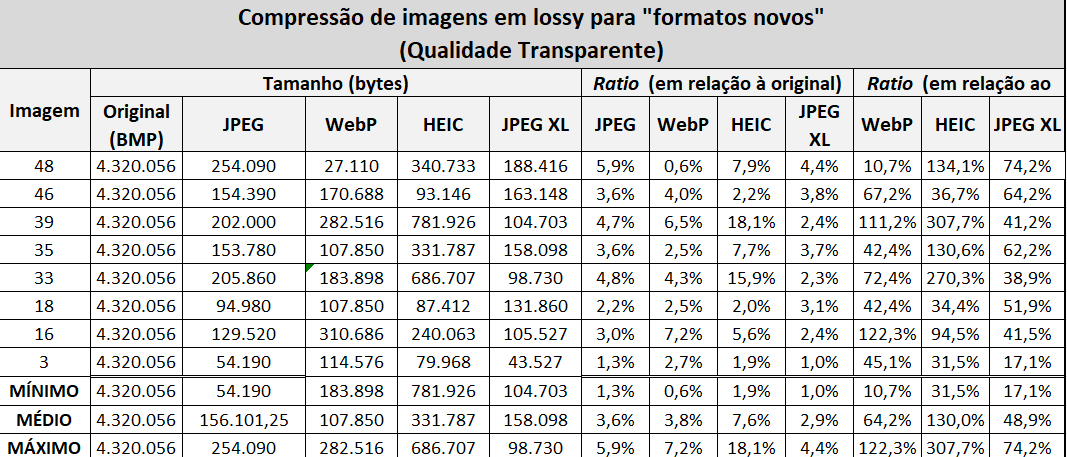
\includegraphics[scale=0.6]{Documeto/1-ElementosTextuais/1-Desenvolvimento/0.png}


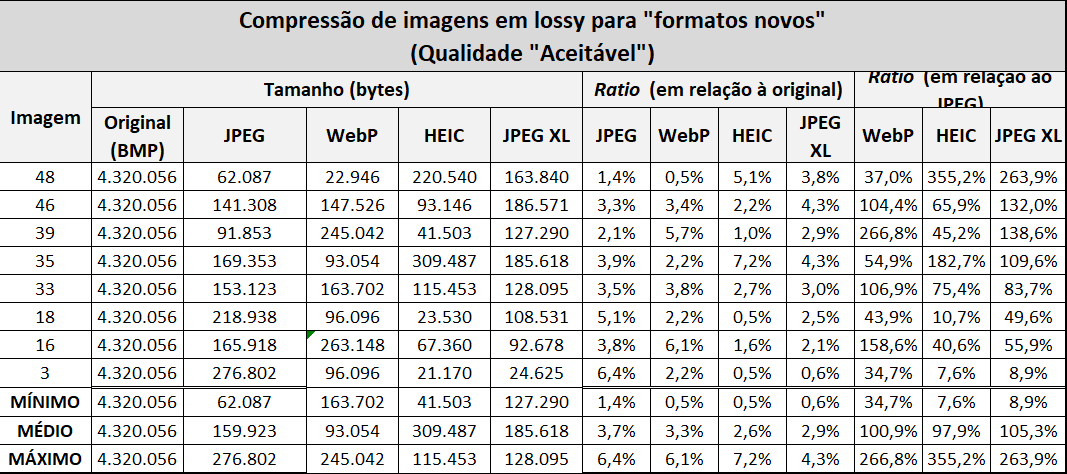
\includegraphics[scale=0.6]{Documeto/1-ElementosTextuais/1-Desenvolvimento/1.png}
    % ----------------------------------------------------------

\captionsetup{justification=centering,margin=0cm}

%inicio do capitulo
\chapter[CONCLUSÃO]{CONCLUSÃO}
\index{CONCLUSÃO}
\label{cap:conclusão}

Após a finalização do trabalho uma série de conhecimentos puderam ser absorvidos. Não só conteúdos importantes para a nossa formação profissional e acadêmica bem como para a nossa vida mesmo. Otimizar o espaço de um hd, escolher a melhor formato de armazenar vídeos, escolher a melhor forma para gravar os vídeos (afinal de constas, se formos subir um vídeo em uma plataforma é melhor que ele seja feito na melhor qualidade para evitar compressões muito desastrosas). Além disso, nossas vidas jamaisserão as mesmas, pois diferente de imagens, os vídeos estão sempre com perdas. Ou seja, cada vídeo no youtube é igual a um ano de vida a menos. 

\url{https://youtu.be/1d_RleeOSyM}


% ----------------------------------------------------------
% ELEMENTOS PÓS-TEXTUAIS (aqueles que estiverem comentados não ão obrigatórios)
% ----------------------------------------------------------


% \printglossary[title=GLOSSÁRIO E ACRÔNIMOS]
% \appendix
\chapter{NOME}
\label{apdc:REF}
TEXTO
% \chapter*{ANEXO A}
\addcontentsline{toc}{chapter}{ANEXO A}
\label{anexo:REF}

% \includepdf[pages=-]{Anexos/nome.pdf} Anexar todas as páginas de um PDF

% \includepdf[pages={X}]{Anexos/nome.pdf} Anexar a página X de um PDF

 
% ANEXAR OUTRAS COISAS, incluindo pdf: NOME DO ANEXO \attachfile[author=name, description=descrição, date=Data, appearance=true, icon=Paperclip]{Anexos/teste.pdf}
% \printindex % CASO QUEIRA USAR O ÍNDICE

\end{document}